%Dokumentklasse

%draft als optionohne bilder für bessere performance
%\documentclass[a4paper,12pt,]{scrreprt}

%normal mit Bildern
\documentclass[a4paper, 11pt, draft=false]{scrartcl}

\usepackage[left= 2.5cm,right = 2.5cm, bottom = 2.5cm,top = 2.5cm]{geometry}

% ============= Packages =============
% Dokumentinformationen
% Standard Packages
\usepackage[utf8]{inputenc}
\usepackage[ngerman]{babel}
\usepackage[none]{hyphenat}
\hyphenpenalty=5000
\tolerance=5000
\providecommand\phantomsection{}
\hyphenation{Brook-field}
\hyphenation{Winkel-ab-wei-chung}
\hyphenation{Stro-mungs-ge-schwin-dig-keit-en}


%Tabellen Packages
\usepackage{makecell}
\usepackage{colortbl}
\usepackage{longtable}
\usepackage{tabularx}
\usepackage{tabulary}
\usepackage{multirow} 

%Grafik Packages
\usepackage{graphicx}
\graphicspath{{img/}}
\usepackage{fancyhdr}
\usepackage{lmodern}
\usepackage[table]{xcolor}
\usepackage{adjustbox}
\usepackage{wrapfig}
\usepackage{svg}

%Diagramm Packages
\usepackage{tikz}
\usetikzlibrary{patterns}
\usepackage{pgfplots}
\pgfplotsset{/pgf/number format/use comma}
\pgfplotsset{grid style={white!90!black}}
\usepackage[edges]{forest}

%Chemie Packages
\usepackage{mhchem}
\usepackage{chemfig}

%Andere Packages
\usepackage{adjustbox}
\usepackage{placeins} %FloatBarrier
\usepackage{booktabs}
\usepackage{caption}
\usepackage[list=true]{subcaption}
\usepackage[shortlabels]{enumitem}
\usepackage{menukeys}
\usepackage{ccicons}
\usepackage{todonotes}

% Mathe Packages
\usepackage{mathtools}
\usepackage{amsfonts}
\usepackage{amsmath}
%Automatisch cdot statt *
\DeclareMathSymbol{*}{\mathbin}{symbols}{"01}
%nur letzte Zeile der Gleichung nummerieren
\makeatletter
\def\Let@{\def\\{\notag\math@cr}}
\makeatother

%Abkürzungsverzeichnis
\usepackage{acronym}

%Seiten Packages
\usepackage{lastpage}
\usepackage{pdfpages}

%Einheitenpackage
\usepackage{eurosym}
\usepackage{siunitx}  
\sisetup{locale = DE, 
	per-mode=fraction,
	inter-unit-product=\ensuremath{\cdot},
	detect-weight = true,
	quotient-mode=fraction
}
%neue Einheiten definieren
\DeclareSIUnit\xyz{xyz}	
\DeclareSIUnit\rpm{rpm}	
\DeclareSIUnit\mws{mWS}	
\DeclareSIUnit\degrees{^\circ}
\DeclareSIUnit\kmeter{\raiseto{3}\meter}
\DeclareSIUnit\seuro{\text{\euro}}
\DeclareSIUnit\hunki{\text{100} \kg}
\DeclareSIUnit\zoll{\text{"}}
\DeclareSIUnit\mpercent{\text{m}\%}
\DeclareSIUnit\umdrehung{U}


\usepackage[
pdftitle={halbautomatische Dosierung eines Assoziativverdickers},
pdfauthor={Roman-Luca Zank},
pdfsubject={Bachelorarbeit zur Erlangung des akademischen Grades Bachelor of Engineering (B. Eng.)},
pdfkeywords={Bachelorarbeit, Dosierung, automatisch, Chemietechnik, Verfahrenstechnik, Assoziativverdicker, Polyurethan, Pumpe},
hidelinks %Entfernt Rahmen von Links
]{hyperref} %immer letztes PAKET !!
	


%========== angepasste Comands ================
%angepasster \today Command
\newcommand{\leadingzero}[1]{\ifnum #1<10 0\the#1\else\the#1\fi}
\newcommand{\todayDE}{\leadingzero{\day}.\leadingzero{\month}.\the\year}

%Tippbox
\newcommand{\tipp}[2]{{
		\textit{#1:}\\
		\vspace*{-5mm}
		\fbox{\parbox{\linewidth}{#2}}}}

%Uhr
\newcommand{\uhr}[2]{#1:#2 Uhr}

%Bild
\newcommand{\bild}[3]{
	\begin{figure}[h!]
		\centering
		\includegraphics[width=#3\textwidth]{img/#2}
		\caption{#1}
		\label{fig:#2}
	\end{figure}
	\FloatBarrier
	\vspace*{-10mm}
}

%Bild in MInipage
\newcommand{\minibild}[3]{
	%\vspace{#3}
	\centering
	\includegraphics[width=#3\textwidth]{img/#2}
	\caption{#1}
	\label{fig:#2}
}

%Anmerkung
\newcommand{\anmerkung}[1]{
	\textcolor{red}{#1}
}

%nicht einrücken nach Absatz
\setlength{\parindent}{0pt}

%Abb. statt Abbildung
\addto\captionsngerman{%
	\renewcommand{\figurename}{Abb.}%
	\renewcommand{\tablename}{Tab.}%
}
	
\newenvironment{parameter}
	{\par\vspace{\abovedisplayskip}\noindent\begin{tabular}{>{$}l<{$} @{${}\ldots{}$} l}}
	{\end{tabular}\par\vspace{\belowdisplayskip}
}

%Ex-Symbol
\newcommand*\exsymbol{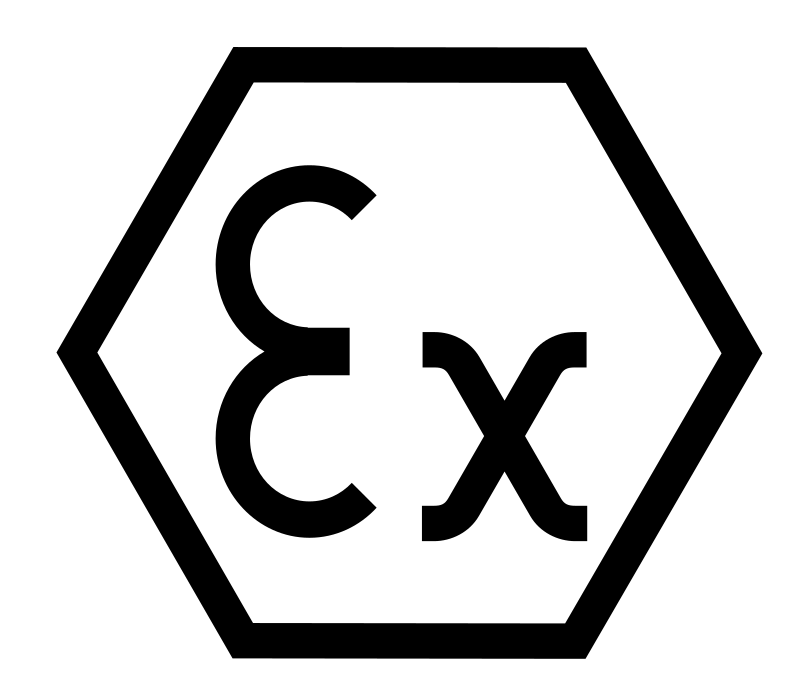
\includegraphics[scale=0.014]{EX-Logo.png}}

%Tabellenfußnote
\newcommand{\tablefootnote}[1]{
	\vspace*{-2.5mm}
	{\footnotesize #1}\\
}




\urlstyle{same}

% ============= Kopf- und Fußzeile =============
\pagestyle{fancy}
%
\lhead{}
\chead{}
\rhead{}%\slshape }%\leftmark}
%%
\lfoot{}
\cfoot{}
\rfoot[{\thepage\ of \pageref*{LastPage}}]{Seite \thepage\ von \pageref*{LastPage}}
%%
\renewcommand{\headrulewidth}{0pt}
\renewcommand{\footrulewidth}{0pt}

%Fußnotelinie
%\let\footnoterule

%Fußnote mit Klammer
\renewcommand*{\thefootnote}{(\arabic{footnote})}

% ============= Dokumentbeginn =============
\begin{document}
	
%Seiten ohne Kopf- und Fußzeile sowie Seitenzahl
\pagestyle{empty}

%\begin{center}
\begin{tabular}{p{\textwidth}}


\begin{center}
	\begin{minipage}{.45\textwidth}
		\centering
		
\includegraphics[scale=0.45]{logos.jpg}\\
	\end{minipage}%
	\begin{minipage}{.55\textwidth}
		\centering
		
\includegraphics[scale=0.45]{logo_unternehmen.jpg}\\
	\end{minipage}
\end{center}

\vspace*{.5mm}

\begin{center}
	\Large{\textsc{Hochschule Merseburg \& Alberdingk Boley Leuna GmbH}}
\end{center}

\vspace*{2.5mm}

\begin{center}
	\Large{\textsc{\textit{Fachbereich Ingenieur- und Naturwissenschaften} }}
\end{center}

\vspace*{5mm}

\begin{center}
	\LARGE{\textsc{\textbf{Bachelorarbeit}}}
	\vspace*{2mm}
	\Large{\textsc{ \\
			zur Erlangung des akademischen Grades \\
			Bachelor of Engineering (B. Eng.) 
	}}
\end{center}

\vspace*{5.5mm}

\begin{center}
	\LARGE{\textit{Thema}:}
\end{center}

\vspace{-5.5mm}

\rule{\textwidth}{0.4pt}
\begin{center}
\textbf{\LARGE{Technische Planung der dosierten Förderung eines hochviskosen Verdickungsmittels}}
\end{center}
\vspace*{-5mm}
\rule{\textwidth}{0.4pt}

\vspace*{13.5mm}

\begin{center}
\Large{\textbf{eingereicht von:}} \\ 
\end{center}
\begin{center}
\Large{Roman-Luca Zank} \\
\end{center}


\vspace*{13.5mm}

\begin{center}
\begin{tabular}{lll}
\Large{\textbf{Betreuer:}}&& \Large{Prof. Dr. nat. techn. Ulf Schubert}\\
&& \Large{Stefan Münch, B.Eng.}\\
&&\\
\Large{\textbf{Kontakt:}}&& \Large{\href{mailto:romanzank@mail.de}{romanzank@mail.de} }\\
\end{tabular}
\end{center}

\end{tabular}
\end{center}

\vfill

\large{Merseburg, \todayDE}


%\include{14_danksagungen}

%\include{15_zusammenfassung}

% Beendet eine Seite und erzwingt auf den nachfolgenden Seiten die Ausgabe aller Gleitobjekte (z.B. Abbildungen), die bislang definiert, aber noch nicht ausgegeben wurden. Dieser Befehl fügt, falls nötig, eine leere Seite ein, sodaß die nächste Seite nach den Gleitobjekten eine ungerade Seitennummer hat. 
%\cleardoubleoddpage

% Pagestyle für Titelblatt leer
\pagestyle{empty}

%Seite zählen ab
\setcounter{page}{0}

%Titelblatt
\begin{center}
\begin{tabular}{p{\textwidth}}


\begin{center}
	\begin{minipage}{.45\textwidth}
		\centering
		
\includegraphics[scale=0.45]{logos.jpg}\\
	\end{minipage}%
	\begin{minipage}{.55\textwidth}
		\centering
		
\includegraphics[scale=0.45]{logo_unternehmen.jpg}\\
	\end{minipage}
\end{center}

\vspace*{.5mm}

\begin{center}
	\Large{\textsc{Hochschule Merseburg \& Alberdingk Boley Leuna GmbH}}
\end{center}

\vspace*{2.5mm}

\begin{center}
	\Large{\textsc{\textit{Fachbereich Ingenieur- und Naturwissenschaften} }}
\end{center}

\vspace*{5mm}

\begin{center}
	\LARGE{\textsc{\textbf{Bachelorarbeit}}}
	\vspace*{2mm}
	\Large{\textsc{ \\
			zur Erlangung des akademischen Grades \\
			Bachelor of Engineering (B. Eng.) 
	}}
\end{center}

\vspace*{5.5mm}

\begin{center}
	\LARGE{\textit{Thema}:}
\end{center}

\vspace{-5.5mm}

\rule{\textwidth}{0.4pt}
\begin{center}
\textbf{\LARGE{Technische Planung der dosierten Förderung eines hochviskosen Verdickungsmittels}}
\end{center}
\vspace*{-5mm}
\rule{\textwidth}{0.4pt}

\vspace*{13.5mm}

\begin{center}
\Large{\textbf{eingereicht von:}} \\ 
\end{center}
\begin{center}
\Large{Roman-Luca Zank} \\
\end{center}


\vspace*{13.5mm}

\begin{center}
\begin{tabular}{lll}
\Large{\textbf{Betreuer:}}&& \Large{Prof. Dr. nat. techn. Ulf Schubert}\\
&& \Large{Stefan Münch, B.Eng.}\\
&&\\
\Large{\textbf{Kontakt:}}&& \Large{\href{mailto:romanzank@mail.de}{romanzank@mail.de} }\\
\end{tabular}
\end{center}

\end{tabular}
\end{center}

\vfill

\large{Merseburg, \todayDE}


% Pagestyle für Rest des Dokuments
\pagestyle{fancy}
\newgeometry{left= 3cm, right = 3cm, bottom = 3cm,top = 3cm}

%Inhaltsverzeichnis
\tableofcontents
%\listoftodos[Noch zu Erledigen]
\thispagestyle{empty}

%Inhalt

\section*{Danksagung}
\label{sec:danksagung}
\section*{Kurzfassung}

\section*{Abstract}
\section*{Eidesstattliche Erklärung}
Hiermit versichere ich, die vorliegende Seminararbeit selbstständig und nur unter Verwendung der von mir angegebenen Quellen und Hilfsmittel verfasst zuhaben. Sowohl inhaltlich als auch wörtlich entnommene Inhalte wurden als solche kenntlich gemacht. Die Arbeit hat in dieser oder vergleichbarer Form noch keinem anderem Prüfungsgremium vorgelegen.\\ \\

Merseburg, den \todayDE \hfill Unterschrift:\rule{6cm}{0,3mm}

\vfill

\section*{Sperrvermerk}
Die vorliegende Arbeit beinhaltet interne vertrauliche Informationen der \linebreak \textsc{\mbox{Alberdingk Boley Leuna GmbH}}. Die Weitergabe des Inhalts der Arbeit im Gesamten oder in Teilen sowie das Anfertigen von Kopien oder Abschriften – auch in digitaler Form -  sind ab dem Abgabedatum der Arbeit untersagt. Ausnahmen bedürfen der schriftlichen Genehmigung der \textsc{\mbox{Alberdingk Boley Leuna GmbH}}. Die Einsichtnahme ist nur dem Verfasser und dem Betreuer zu erlaubt. \\ \\

Merseburg, den \todayDE 

\vfill

\section{Einleitung}
\label{sec:einleitung}
%Warum und was haben Sie untersucht ?
%eine Seite

%Dosierung
%Verdickermittel
%Industrie 4.0

 
In der produzierenden Chemie sind eine Reihe von Verfahrenschschritten notwendig um das gewünschte Zielprodukt herzustellen. Für die Produktion von Polymerdispersionen der Farben-, Lack- und Beschichtungsindustrie ist das Fördern von Basischemikalien wie organischen und anorganischen Säuren und Basen, Lösemitteln, Initiatoren, Emulgatoren und Additven elementar. Gerade Additive werden oft in geringen Mengen mit hoher Wirksamkeit eingesetzt, weshalb das Verfahren der Dosierung anzuwenden ist. 
 
\section{Zielsetzung und Abgrenzung der Aufgabenstellung}
\label{sec:aufgabenstellung}
%eine Seite
%----------
%Motivation --> Ohrenöffner
%zentrale Frage
%Aufbau, Vorgehensweise, Methoden

\subsection{Zielsetzung der Aufgabenstellung}

\subsection{Abgrenzung der Aufgabenstellung}

\section{Theoretische Grundlagen}
\label{sec:grundlagen}
%zugrundeliegende Theorien und Modelle
% Definitionen
% Stand der Technik, Normen und Standards, Wirtschaftliche Aspekte
% persönliche Positionierung


\todo[inline]{Optional Stand der Technik betrachten --> Fassfolgeplatten Systeme}

\subsection{Chemische Produktion und Prozesssicherheit}
Es gibt verschiedene Charakteristika, die den Betrieb einer chemischen Anlage beschreiben. Dazu gehören zum einen die technische Ausführung der Verfahrenstechnik, aber auch Aspekte wie die Arbeitsweise der Produktion oder das vorliegende Sicherheitskonzept.

\subsubsection{Produktionsweisen in der Chemie}
Chemieanlagen können je nach Produkt und Produktionsmenge auf verschiedene Weisen produzieren. 

\paragraph{Batch-Betrieb} Eine Arbeitsweise der chemischen Produktion stellt der sogenannte Batch-Betrieb, auch Chargenbetrieb genannt, dar. Bei dieser Fahrweise werden jegliche Prozess- und Verfahrensschritte in zeitlich festgelegter Reihenfolge nacheinander durchgeführt. Die Ausgangsstoffe werden hierfür in ein geeignetes Reaktionsgefäß, wie zum Beispiel einen Rührkessel, gegeben und die Reaktion gestartet. Danach wird das Reaktionsprodukt in entsprechende Lagertanks oder Gebinde transferiert und das Reaktionsgefäß gereinigt.\linebreak
Gerade für geringe Produktionsmengen oder häufigerem Wechsel der Produkte wird diese Betriebsweise bevorzugt. Durch den variablen Aufbau der Anlage werden somit auch verschiedene Reaktionszeiten und Herstellungsverfahren möglich gemacht.\,\cite{Ignatowitz.2015}\linebreak
In der Produktionsplanung einer solchen Produktionsweise können mehrerer Batches auf einer Fertigungslinie für das selbe Produkt geplant werden. Die Zusammenfassung dieser Batches wird allgemein als Produktionskampagne bezeichnet und hat den Vorteil, dass mehrere Batches hintereinander gefahren werden und somit weniger Unterbrechungen durch mögliche Umrüst- oder Reinigungsarbeiten entstehen. Zudem lassen sich bei der Lagerung einer Kampagne durch die einzelnen Batches Produktionsabweichungen ausgleichen.\,\cite{SAP.04.02.2022}

\paragraph{Kontinuierlicher Betrieb} Dem Batch-Betrieb gegenüber steht der kontinuierliche Betrieb. Im Gegensatz zur zeitlichen Taktung von Batch-Anlagen findet für diese Arbeitsweise eine örtliche Separierung der Verfahrensschritte bei kontinuierlichem Massenstrom statt. Die Prozessbedingungen, wie Temperatur, Druck oder Produktzusammensetzung sind deshalb stationär. Durch den festen Reaktionsablauf der Anlage eignet sich diese Fahrweise hauptsächlich für große Produktionsmengen. Neben dem Hauptprodukt fallen für diese Produktionsweise natürlich auch mögliche Nebenprodukte kontinuierlich an und sind entsprechend zu verwerten. \cite{Ignatowitz.2015}


\subsubsection{Industrielle Gebinde für Flüssigkeiten}
Um ein Edukt neu in die Produktion einzubinden sind, nicht nur die chemisch-physikalischen Eigenschaften relevant. Auch der Aspekt der Gebindeform ist maßgeblich für die Einfügung des Eduktes in den Produktionsablauf. Für flüssige Edukte sind im Tagesgeschäft der \textsc{Alberdingk Boley Leuna GmbH} hauptsächlich Kunststoff-IBCs (Intermediate Bulk Container) und zum Teil Kunststoff-Deckelfässer im Einsatz. Es sei jedoch erwähnt, dass auch weitere Gebinde auf dem Verpackungsmarkt verfügbar sind, wie beispielsweise Flüssig-IBCs, Kanister, Hobbocks oder Metallfässer.\\
Den IBC als kubisches Gebinde gibt ca. seit den 1960er Jahren  und hat sich über eine Richtlinie des VDI aus den frühen 70er-Jahren zu einem Standard der großen Einzelverpackungen entwickelt. Zuvor waren zum Großteil \SI{200}{\liter}-Fässer im Einsatz, welche sich neben der geometrischen Form auch maßgeblich im Handling zum IBC unterscheiden. \cite{neueverpackung.01.02.2022}
So lassen sich Fässer in dieser Größenordnung beispielsweise vorwiegend als 4er-Packung sicher transportieren und benötigen hierfür zusätzliche Paletten, sowie Schrumpffolie oder Transportbänder um die Behälter zu fixieren. Ein IBC hingegen kann direkt als Gebinde mit einem Hubwagen oder Gabelstapler transportiert werden ohne umfangreiche Vorbereitung. Weitere Punkte im Vergleich zwischen IBC und Fass finden sich unter Tabelle \ref{tab:ibc_fass}.

% Table generated by Excel2LaTeX from sheet 'Daten'
\begin{table}[h!]
	\renewcommand*{\arraystretch}{1.2}
	\centering
	%\rowcolors{2}{white}{gray!25}
	\caption{Allgemeiner Vergleich der Gebinde IBC und Fass \cite{MakrusKamroth.01.02.2022}}
	\label{tab:ibc_fass}
	\resizebox{\textwidth}{!}{
		\begin{tabulary}{1.0\textwidth}{C|C|C|C}
			\hline
			\textbf{} 						& \textbf{Einzelfass (1 Fass)} 			& \textbf{Fasspalette \linebreak (4 bis 5 Fässer)} & \textbf{IBC \linebreak (1 Container)}\\
			\hline
			\textbf{UN-Zertifikat} 		&	\multicolumn{3}{c}{möglich} \\
			\hline
			\textbf{Transportvorbereitung} 	& \multicolumn{2}{c|}{\parbox{6cm}{\centering \, \newline evtl. extra Palette mit Schrumpffolie/Transportbänder}}  & \parbox{3cm}{\centering \, \newline keine}\\
			\hline
			\textbf{Transport \linebreak (voll)} 				& schwer \linebreak mit Fassheber 	&\multicolumn{2}{c}{\parbox{6cm}{\centering \, \vspace*{2mm} \newline Gabelstapler, Flurförderzeuge}}\\
			\hline
			\textbf{Transport \linebreak (teilentleert)} 		& schwer \linebreak mit Fassheber 	& schwer mit Gabelstapler, Flurförderzeuge & Gabelstapler, Flurförderzeuge\\
			\hline
			\textbf{Abfüllmenge} 			& klein							& klein bis mittel				& mittel bis groß \\
			\hline
			\textbf{Lagerkapazität} 		& sehr klein			& klein	bis mittel				& groß\\
			\hline
			\parbox{3cm}{\, \vspace*{2mm} \newline \textbf{Erwärmbarkeit}}			& \parbox{2cm}{\centering \, \vspace*{2mm} \newline möglich}	 & \parbox{4cm}{\centering\, \vspace*{2mm} \newline nicht möglich}	 & möglich, \linebreak aber nicht effektiv\\
			\hline
			\textbf{Verwendung} 			& \multicolumn{2}{c|}{i.d.R einmalig} & mehrmals möglich\\
			\hline
			\textbf{Stapelbarkeit} 			& \multicolumn{2}{c|}{schlecht stapelbar} & gut stapelbar\\
			\hline
			\textbf{Produktreste} 		& \multicolumn{2}{c|}{$>\SI{5}{\kg}$}&$\leq\SI{5}{\kg}$\\
			\hline	
			\textbf{Anschlüsse} 		& \multicolumn{2}{c|}{Deckel oder Spundloch} & Deckel oder Auslaufarmatur	\\
			\hline
		\end{tabulary}
	}
\end{table}%
\FloatBarrier

\subsubsection{Sicherheit von Chemieanlagen}
Das Thema Sicherheit findet sich neben dem Gefahrguttransport in der Logistik natürlich auch im restlichen Umfang der Chemieanlage wieder. 
Vom Betreiber einer solchen Anlage ist durch verschiedene Gesetzte, Verordnungen und technischen Regeln ein Gesamtsicherheitskonzept zu erarbeiten und umzusetzen. Beispiele solcher Gesetze sind das Arbeitsschutzgesetzt, das Chemikaliengesetz, das Umweltverträglichkeitsgesetz und das Geräte- und Produktionssicherheitsgesetz GSPG. \linebreak 
Diese Gesetze münden dann seit dem Jahr 2002 in die Betriebssicherheitsverordung (kurz: BetrSichV), welche eine Gesamtbetriebssicherheitsverordnung darstellt und die eben genannten Gesetzte zusammenfasst. Weitere zu beachtende Verordnungen sind die Explosionsschutz- und die Gefahrstoffverordnung.\linebreak
Aus diesen Verordnungen setzten sich nun wiederum verschiedenste technische Regeln wie die EU-Richtlinie 94/9/EG (ATEX 100a), Technische Regeln für Behälter (TRB) oder Technische Regeln für Rohrleitungsanlagen (TRR) zusammen. Diese erleichtern das Umsetzen, der geforderten Verordnungen und Gesetze und bilden zusammen mit berufsgenossenschaftlichen Regelungen ein Gesamt-Sicherheitskonzept für eine chemische Anlage. \cite{Ignatowitz.2015}\\
Ausführung eines solchen Sicherheitskonzeptes in der Praxis zeigt sich zum Beispiel in Form von Arbeits- und Betriebsanweisungen für die Mitarbeiter. Aber auch regelmäßige Sicherheitsschulungen, Instandhaltung der Anlage, Nutzung sicherheitstechnischer Ausrüstung, Dimensionierung und Ausführung der Verfahrenstechnik, Ausweisung von Explosionszonen und viele weitere Punkte ergeben sich aus diesem festgelegten Sicherheitskonzept. Für weiterführende Informationen sei an dieser Stelle auf die angegebenen Verordnungen verwiesen. Für einen Überblick über die Thematik lassen sich weitere Informationen in \cite{Ignatowitz.2015} finden.

\paragraph{Zoneneinteilung explosionsgefährdeter Anlagenbereiche gemäß ATEX 137}
Da das Sicherheitskonzept der \textsc{Alberdingk Boley Leuna GmbH} ebenfalls die Einteilung von Explosionszonen beinhaltet, wird die EU-Richtlinie 1999/92/EG (ATEX 137) in kurzer Form näher erläutert. Die Prüfung eines Bereiches auf eine explosionsgefährdete Zone erfolgt durch eine sicherheitstechnische Fachkraft. Wird der Bereich als explosionsgefährdet eingestuft, ist eine Festlegung auf die Zone 0, Zone 1 oder Zone 2 möglich. Diese unterscheiden sich im Ausmaß der Explosionsgefährdung in diesem Bereich.\linebreak
Nach ATEX 137 stellt Zone 2 der explosionsgefährdeten Bereiche den Bereich mit der geringsten Explosionsgefahr da. Im Normalbetrieb ist nicht davon auszugehen, dass eine explosionsfähige Atmosphäre entsteht und wenn dann nur kurzzeitig in Erscheinung tritt. Beispiele hiefür können Produktionsbereiche sein in denen mit brennbaren Flüssigkeiten hantiert wird. Zudem gehören Bereiche, welche die Zonen 1 und 0 näher umgeben ebenfalls zur Zone 2.\linebreak
Die Zone 1 beschreibt den nächsthöheren Grad der explosionsgefährdeten Bereiche. In dieser Zone treten im Normalbetrieb gelegentlich explosionsfähige Atmosphären als Gemisch aus brennbaren Gasen, Dämpfen oder Nebeln und Luft auf. Zu dieser Zone gehören jegliche Bereiche in nähere Umgebung zu Zone 0, aber auch zum Teil das innere von Reaktionsgefäßen, der nähere Bereich von leicht zerbrechlichen Armaturen (z.B. aus Glas) oder der Raum um Beschickungsöffnungen und Abfüllanlagen.\linebreak
Bereiche mit der größten Explosionsgefährdung werden mit Zone 0 bezeichnet. Hier sind explosionsfähige Atmosphären aus Luft und brennbaren Stoffen (Gase, Nebel, Dämpfe) häufig oder über längere Zeiträume vorzufinden. Meist werden die Bedingungen für diese Zone nur von Inneren von Behältern, Rohrleitungen oder Anlagen bedient.

%Weiterhin sind folgende Punkte zu beachten
%\begin{itemize}
%	\item sicherheitstechnische Ausrüstung (z.B. Sicherheitsventile, Gasmessgeräte, ...) ist bereitzustellen und zu nutzen
%	\item Sicherstellung von Wissen über die genutzten Gefahrstoffe und Vorgänge, sowie deren Beherrschung
%	\item Verfahrenstechnik in der Anlage ist sicherheitstechnisch einwandfrei auszulegen und überprüfen zu lassen
%	\item die Anlagendimensionierung sollte den genutzten Betriebsbedingungen und Chemikalien entsprechen und mit Sicherheitszuschlägen versehen werden
%	\item Sicherheit ist durch Instandhaltung der Anlage zu gewährleisten
%	\item Es sind EMSR und PLT-System zur Überwachung und Meldung von Störfällen in der Anlage zu nutzen
%	\item die Anlage ist mit qualifiziertem Personal in ausreichender Anzahl zu fahren
%	\item das an und in der Anlage arbeitende Personal hat sich regelmäßigen Sicherheitsunterweisungen zu unterziehen
%\end{itemize}


\todo[inline]{Beschreibung Sicherheit in Chemieanlagen mit Explosionszone etc.}

\subsection{Definition und Gliederung zu Verdickungsmitteln}

In der Farben- und Putzindustrie werden Verdickungsmittel als rheologische Additive bezeichnet. Sie erhöhen die Viskosität von Flüssigkeiten und ändern somit ihre rheologischen Eigenschaften, welche die Auftragungs-, Fließ- und Verlaufseigenschaften von Farben und Putzen bestimmen. Verdickungsmittel kommen jedoch auch in der Lebensmittelchemie oder Pharmazie zum Einsatz. Je nach dem welche Anforderungen an das Verdickermittel gestellt werden, unterscheiden sich diese in ihrer Zusammensetzung (siehe Abb. \ref{fig:verdicker_einteilung}). \cite{Brock.2009}

\begin{figure}[h!]
	\centering
	\begin{forest}
		forked edges,
		for tree={draw,align=center,edge={-latex}}
		[Verdickungsmittel, for children={fit=band}
		[Anorganisch]
		[Organisch, for children={fit=band}
		[Niedermolekular]
		[Synthetisch]
		[Natürlich, for children={fit=band}
		[Natürlich (abgewandelt)]
		]	
		]	
		]
	\end{forest}	
	\caption{Einteilung von Verdickungsmitteln nach Zusammensetzung \cite{Brock.2009}}
	\label{fig:verdicker_einteilung}
\end{figure}
\FloatBarrier

Je nach Verdickungsmittel können verschiedene Effekte wie Gelbildung, Solvatation, Ausbildung von Netzstrukturen, Coulomb-Kräfte, Quellung und Wasserstoff- Brückenbindungen, sowie deren gegenseitige Einflussnahme die Erhöhung der Zähflüssigkeit bewirken. \cite{Brock.2009} \\
Betrachtet man speziell die sogenannten assoziativen Verdickungsmittel lassen sich diese den Gruppen der abgewandelten, natürlichen Verdicker und den synthetischen Verdickern zuordnen.  Sie spezifizieren sich gegenüber anderen Verdickertypen darin, dass sie neben hydrophilen Gruppen auch hydrophobe End- und Seitengruppen enthalten, welche dem Verdickungsmittel einen Tensidcharakter verleihen. Deshalb bestehen assoziative Verdicker unteranderem aus hydrophob modifizierten Polymerstrukturen (siehe Abb. \ref{fig:assoziativ_einteilung}).

\begin{figure}[h!]
	\centering
	\begin{forest}
		forked edges,
		for tree={draw,align=center,edge={-latex}}
		[Assoziativverdicker
		[hydrophob \\ modifizierte \\ Polyacrylate]
		[hydrophob \\ modifizierte \\ Celluloseether]
		[hydrophob \\ modifizierte \\ Polyether]
		[hydrophob \\ modifizierte \\ Polyacrylamide]
		[assoziative \\ Polyurethan-Verdicker]
		]
	\end{forest}	
	\caption{Einteilung von Assoziativ-Verdickern nach chemischer Struktur \cite{Brock.2009}}
	\label{fig:assoziativ_einteilung}
\end{figure}
\FloatBarrier
Diese strukturelle Eigenschaft der Assoziativ-Verdicker macht die Bildung von Micellen möglich und es treten neben der Quellung in der Wasserphase sogenannte "`Micellbrücken"' zwischen Latex-Teilchen der Bindemitteldisperion auf, welche eine zusätzlich Viskositätserhöhung bewirken. \cite{Brock.2009} \\
In Abbildung \ref{fig:struktur_puverdicker} ist eine schematische Struktur eines solchen assoziativen Polyurethan-Verdickers aufgeführt. Diese beispielhafte Struktur zeigt hydrophile, höher molekulare Polyethersegmente, welche über Urethan-Gruppen verbunden sind und durch hydrophobe Molekülgruppen verknüpft werden. \cite{Brock.2009}

\begin{figure}[h!]
	\centering
	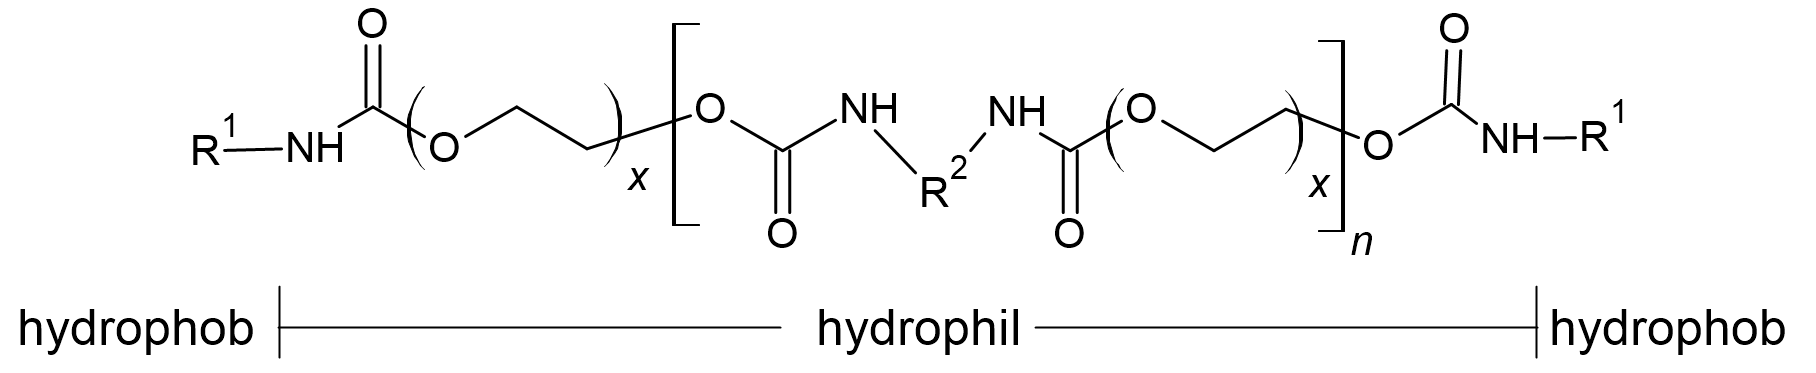
\includegraphics[width=0.75\textwidth]{img/verdicker_struktur}
	\caption{schematische Struktur eines assoziativen Polyurethan-Verdickers, \linebreak erstellt nach \cite{Brock.2009}}
	\label{fig:struktur_puverdicker}
\end{figure}
\FloatBarrier

Durch diesen Mix der hydrophoben und hydrophilen Strukturen wird der Tensidcharakter des Verdickungsmittels bestimmt und es ergeben sich Netzstrukturen mit assoziierten "`Micellbrücken"', wie in Abbildung \ref{fig: verdicker_anwendung} dargestellt. Zusätzlich ist zu erkennen, dass auch Wechselwirkungen mit bereits vorhandenen Tensidmolekülen in der Dispersion auftreten können und die Struktur somit weiter stabilisieren. \cite{Mezger.2016}

\begin{figure}[h!]
	\centering
	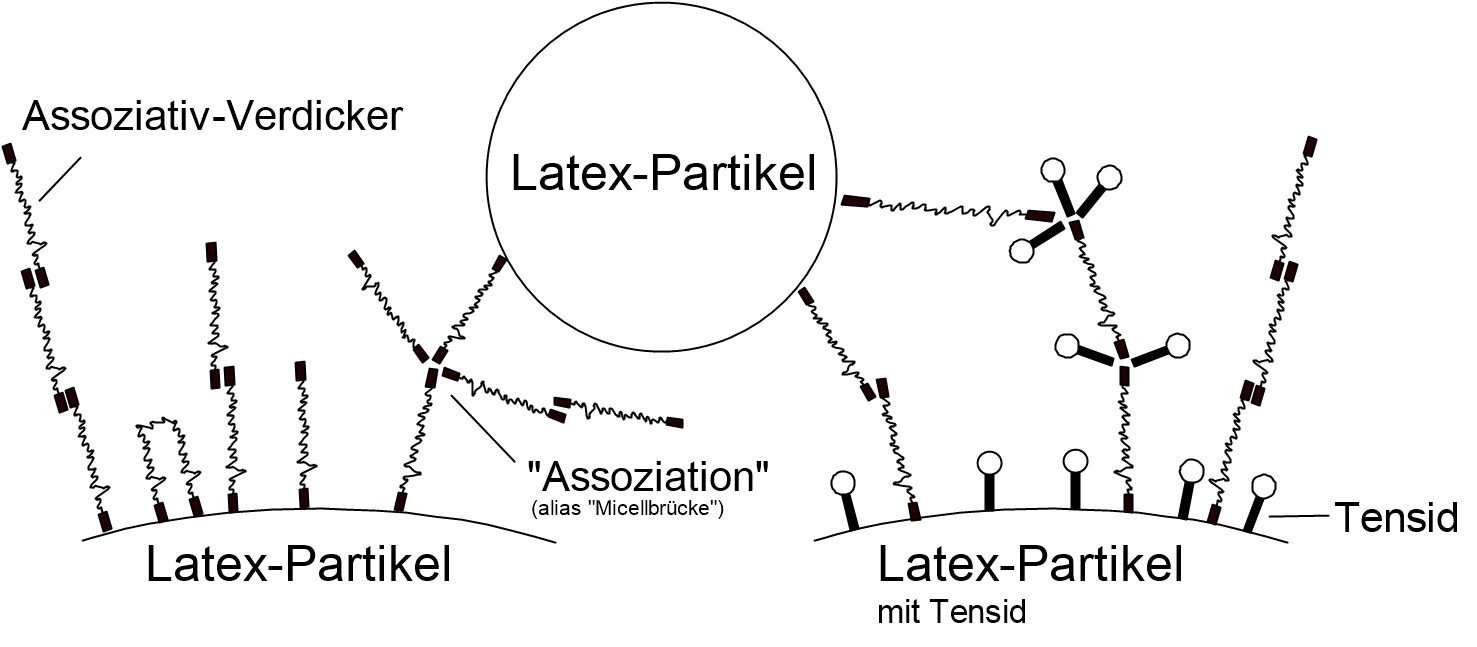
\includegraphics[width=0.75\textwidth]{img/verdicker_anwendung}
	\caption{Netzstruktur durch Verdickermittel in Latex-Dispersion (mit und ohne Tensid), \linebreak erstellt nach \cite{Mezger.2016}}
	\label{fig: verdicker_anwendung}
\end{figure}
\FloatBarrier

Aufgrund dieser ausgeprägten Netzstrukturen innerhalb des Verdickungsmittels ist es jedoch auch möglich, dass das Verdickungsmittel selbst eine hohe Viskosität aufweist. Dieser Punkt kann erheblichen Einfluss auf die großtechnische Verarbeitbarkeit des Additives haben und wird im weiteren Verlauf dieser Arbeit näher betrachtet. 

\subsection{Dosierung von Flüssigkeiten}

\subsubsection{Charakterisierung des Dosierstroms}
\paragraph*{Rheologie von Fluiden} Um den Dosierstrom einer Flüssigkeit charakterisieren,  ist es zunächst nötigt die Fließeigenschaften beschreiben zu können. Die Wissenschaft der Rheologie beschäftigt sich unter anderem mit dem Fließ- und Deformationsverhalten von Flüssigkeiten und teilt diese zunächst in \textsc{Newtonsche} und \textsc{Nichtnewtonsche} Fluide ein. Grundlage dieser Einteilung sind Untersuchungen von \textsc{Isaac Newton}, welcher sich bei konstanter Temperatur mit der Schergeschwindigkeit $D$ in Abhängigkeit von der Schubspannung $\tau$ beschäftigte. 
Das Ergebnis dieser Arbeit ist das \textsc{Newtonsche Fließgesetz} unter Gleichung \eqref{eq: newton}, welche den Fließwiderstand $\eta$ einer Flüssigkeit bei gegebener Temperatur als Stoffkonstante benennt. Dieser Fließwiderstand $\eta$ ist heute unter der Bezeichnung der dynamischen Viskosität bekannt.

\begin{equation}
	\label{eq: newton}
	\tau = \eta * D
\end{equation}
\begin{parameter}
	D 			& Schergeschwindigkeit\\
	\tau 		& Schubspannung\\
	\eta 		& Dynamische Viskosität\\
\end{parameter}

Es sei erwähnt, dass neben der dynamischen Viskosität auch eine kinematische Viskosität $\nu$ existiert. Diese beschreibt in Gleichung \eqref{eq:kivisko} jedoch lediglich das Verhältnis zwischen der dynamischen Viskosität und der Dichte eines Fluides.

\begin{equation}
	\label{eq:kivisko}
	\nu = \frac{\eta}{\rho}
\end{equation}
\begin{parameter}
	\nu 		& kinematische Viskosität\\
	\rho 		& Dichte\\
	\eta 		& Dynamische Viskosität\\
\end{parameter}

Schlussendlich gilt für die Einteilung der Fluide nach Gleichung \eqref{eq: newton}, dass alle Fluide, welche eine Linearität zwischen Schergeschwindigkeit und Schubspannung ohne Fließgrenze aufweisen als \textsc{Newtonsche} Fluide und diejenigen, die ein nicht-lineares Verhalten und/oder ein Verhalten mit Fließgrenze aufweisen als \textsc{Nichtnewtonsche} Fluide eingeordnet werden. Veranschaulicht wird dies in Abbildung\,\ref{fig: arten_fluide} mit einer Auswahl an verschiedenen Rheologieprofilen.

\begin{figure}[h!]
	\begin{minipage}[b]{0.475\textwidth}
		\centering
		\includegraphics[width=\textwidth]{img/fluidarten}
		\caption{Fließkurven für verschiedene \linebreak Fluide, erstellt nach \cite{Holze.2010}}
		\label{fig: arten_fluide}
	\end{minipage}
	\hspace*{0.05\textwidth}
	\begin{minipage}[b]{0.475\textwidth}
		\centering
		\includegraphics[width=\textwidth]{img/fluidarten2}
		\caption{Viskositätskurven für verschiedene Fluide, erstellt nach \cite{MunzingChemieGmbH.2018}}
		\label{fig: arten_fluide2}
	\end{minipage}
\end{figure}
\FloatBarrier

%\paragraph*{Messmethoden zur Viskositätsbestimmung}
Zur Bestimmung der Viskosität müssen für ein \textsc{Newtonsches} Fluid laut Gleichung\,\eqref{eq: newton} die Schergeschwindigkeit $D$ und die Schubspannung $\tau$ bestimmt werden. Eine Möglichkeit hierfür ist die Nutzung eines sogenannten Rotationsviskosimeters. Allgemein beschreiben Rotationsviskosimeter einen Viskosimetertypen, bei dem die zu messende Flüssigkeit zwischen spezifisch geformten Körpern gebracht wird, von denen einer rotiert. Dabei tritt eine Scherung der Flüssigkeit auf und das aufgewendete Drehmoment am Viskosimeter wird gemessen. Neben Rotationsviskosimetern sind auch weitere Viskosimetertypen wie Kappilarviskoskosimeter und Fallkörperviskosimeter bekannt. Diese unterscheiden sich neben dem Aufbau gegenüber dem Rotationsviskosimeter beispielsweise auch darin, dass sie im Regelfall die Viskosität von \textsc{Nichtnewtonschen} Fluiden nicht ausreichend untersucht werden kann. \cite{ROMPPRedaktion.2008}

\paragraph*{Bestimmung der Strömungsform} Nachdem die Viskosität bestimmt ist, lässt sich nun der Dosierstrom des Verdickermittels entsprechend seiner Strömungseigenschaften beschreiben. Hier für wird die sogenannte \textsc{Reynoldszahl} bestimmt. Sie ist eine dimensionslose Kennzahl und beschreibt das Verhältnis zwischen Trägheitskräften zu Reibungskräften in strömenden Flüssigkeiten und ist für durchströmte Rohrleitungen unter Gleichung\,\eqref{eq: reynolds} definiert. \cite{Foth.2014}

\begin{equation}
	\label{eq: reynolds}
	Re = \frac{d_H*\rho*\overline{u}}{\eta}
\end{equation}
\begin{parameter}
	Re 			& 	\textsc{Reynoldszahl} \\
	\eta 		& dynamische Viskosität des Fluids\\
	\rho 		& Dichte des Fluids\\
	d_H			&	hydraulischer Rohrdurchmesser\\
	\overline{u} & mittlere Strömungsgeschwindigkeit\\
\end{parameter}

Anhand der \textsc{Reynoldszahl} lässt sich nun mithilfe der Tabelle \ref{tab:stromung_reynolds}, die jeweilige Strömungsform zuordnen. Diese Zuordnung ist wichtig, da sich je nach Strömungsform unterschiedliche Einflussgrößen auf den Druckverlust somit auf die Auslegung der Dosierung ergeben. Beispielsweise hat für eine laminare Strömung die Wandrauigkeit der Leitung keinen Einfluss mehr, wohin gegen sie in turbulenten Strömungen maßgebliche Druckverluste hervorrufen kann. In laminaren Strömungen überwiegt hierbei der glättende Einfluss der Viskosität gegenüber den Rohrunebenheiten, während in turbulenten Strömungen weitere Wirbel erzeugt werden. \cite{Bschorer.2018}

% Table generated by Excel2LaTeX from sheet 'Daten'
\begin{table}[h!]
	\renewcommand*{\arraystretch}{1.2}
	\centering
	\caption{Strömungsformen und ihre Reynoldszahlen \cite{Foth.2014}}
	\label{tab:stromung_reynolds}
	%\resizebox{10.5cm}{!}{
		\begin{tabulary}{1.0\textwidth}{C|CCC}
			\hline
			\textbf{Strömungsform} & \textbf{Laminar} & \textbf{instabiler Bereich} & \textbf{Turbulent}\\
			\hline
			\textbf{Reynoldszahl} &	$< 2300$ & $2300$ bis $4000$& $>4000$\\
			\hline			
		\end{tabulary}
		%}
\end{table}%
\FloatBarrier

Nach der Bestimmung der Reynoldszahl lässt sich nun mit Hilfe des \linebreak \textsc{Nikuradse-Colebrook-Moody}-Diagramms, nachfolgend \textsc{Moody}-Diagramm genannt, die Rohrreibungszahl $\lambda$ bestimmen (siehe Abb. \ref{fig:moody}). Diese Rohrreibungszahl ist eine dimensionslose Kennzahl und kann zweckmäßig in Gleichung \eqref{eq:druckverlustbeiwert} eingesetzt werden. Somit ist es möglich den dimensionslosen Druckverlustbeiwert $\zeta_R$ für gerade Rohrleitungen zu bestimmen und ermöglicht daraufhin die Berechnung des durch Reibung verursachten Druckverlustes $\Delta p$ auf Basis der erweiterten \textsc{Bernoulli}-Gleichung \eqref{eq:druckverlust_zeta}. \cite{Bschorer.2018}

\begin{equation}
	\label{eq:druckverlustbeiwert}
	\zeta_R = \lambda * \frac{L}{d}
\end{equation}
\begin{equation}
	\label{eq:druckverlust_zeta}
	\Delta p = \frac{1}{2}*\zeta_R*\rho*\overline{u}^2
\end{equation}
\begin{parameter}
	\zeta_R		& Druckverlustbeiwert für gerade Rohrstrecken\\
	L 			& Rohrleitungslänge\\
	d			& Rohrdurchmesser\\
	\Delta p	& Druckverlust \\
	\rho 			& Dichte des Fluids\\
	\overline{u} 	& mittlere Strömungsgeschwindigkeit\\
\end{parameter}


\begin{figure}[h!]
	\centering
	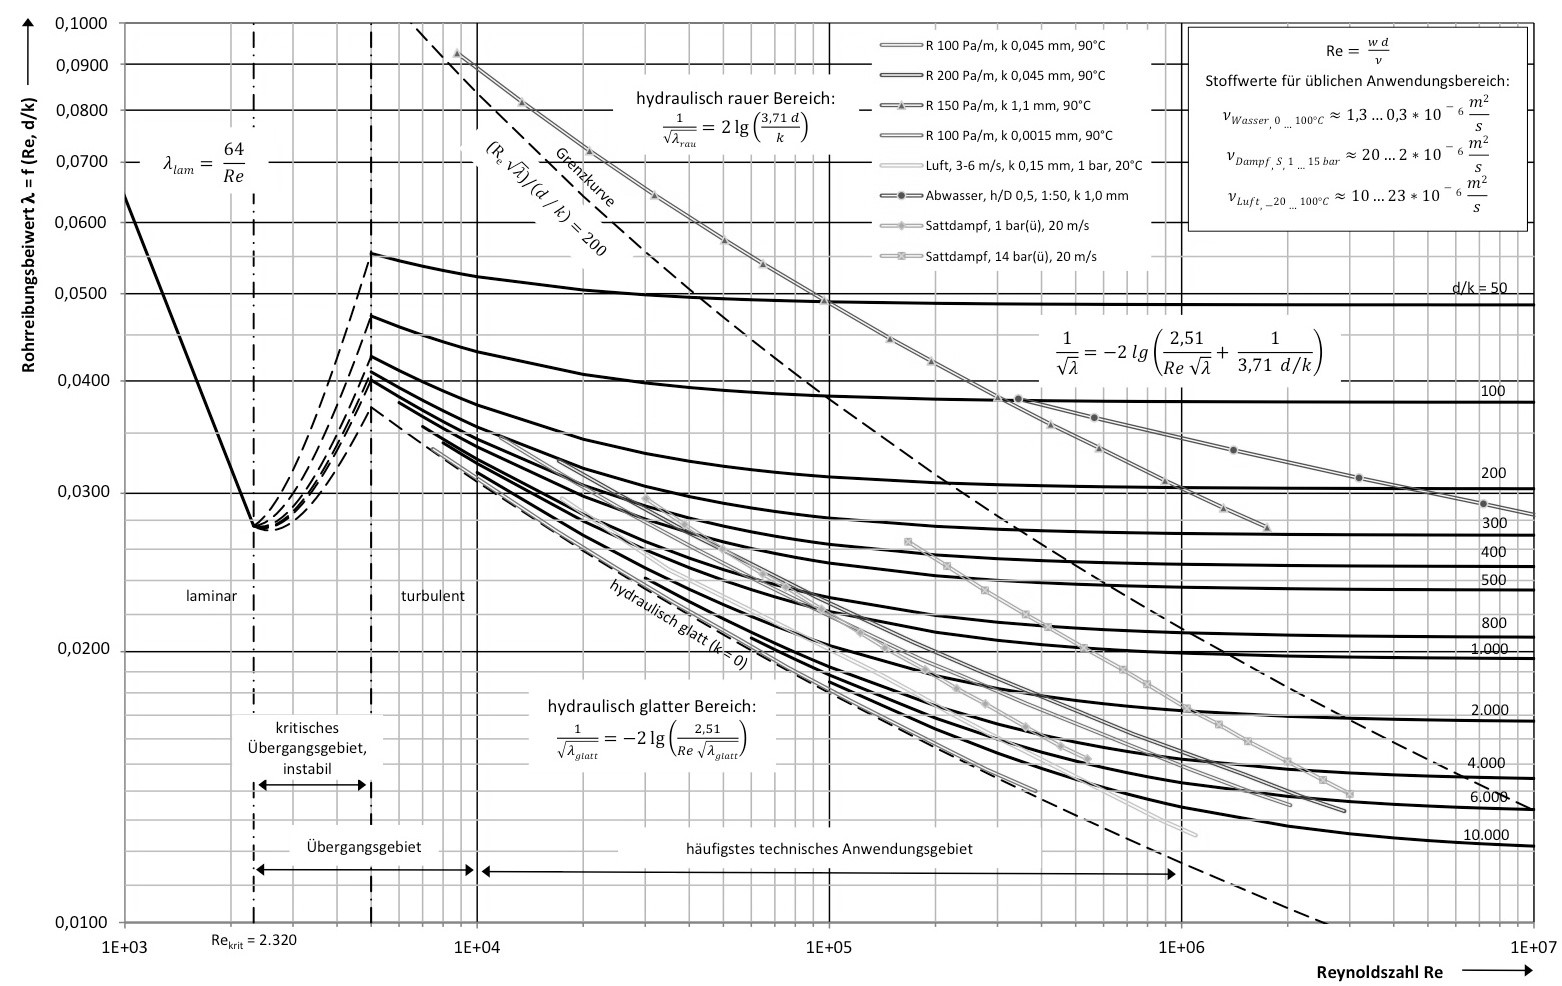
\includegraphics[width=1.0\textwidth]{img/R_Rohrreibungsbeiwert.jpg}
	\caption{\textsc{Nikuradse-Colebrook-Moody}-Diagramm \cite[\ccbysa]{Msimca.2017}}
	\label{fig:moody}
\end{figure}
\FloatBarrier
%Ende

\paragraph*{Gesetz von  \textsc{Hagen}-\textsc{Poiseuille}} Liegt für eine nicht-kompressible Flüssigkeit eine laminare Strömung vor, so ist es möglich die zuvor beschriebene Vorgehensweise zu vereinfachen und den auftretenden Druckverlust in einer geraden Rohrleitung direkt mit dem Gesetz von \textsc{Hagen}-\textsc{Poiseuille} zu bestimmen.  Der Druckverlust wird hierbei in Abhängigkeit vom Volumenstrom, der Rohrleitungslänge, des Rohrdurchmessers und der Viskosität berechnet. Die Definition des Gesetzes, aufgelöst nach dem Druckverlust, findet sich unter Gleichung \eqref{eq:hagen}. \cite{Foth.2005}

\begin{equation}
	\label{eq:hagen}
	\Delta p  = \frac{8*\eta*L*\dot{V}}{r^4*\pi}
\end{equation}
\begin{parameter}
	\Delta p	& Druckverlust \\
	\eta 		& dynamische Viskosität des Fluids\\
	\dot{V}		& Volumenstrom des Fluids\\
	r			& innerer Radius der Rohrleitung\\
	L 			& Rohrleitungslänge\\
\end{parameter}

Da das Gesetz von \textsc{Hagen}-\textsc{Poiseuille} bereits im \textsc{Moody}-Diagramm enthalten ist, können beide Vorgehensweisen genutzt werden um die jeweils andere Rechnung zu überprüfen. Sollen Rohrleitungseinbauten wie Armaturen, Ventile oder Bogenstücke einberechnet werden, vereinfacht jedoch aufgrund von tabellierten Druckverlustbeiwerten möglicher Einbauten die erweiterte \textsc{Bernoulli}-Gleichung die Berechnung des gesamten reibungsbedingten Druckverlustes.

\subsubsection{Dosierpumpen}
Da Flüssigkeiten keine hohen Abweichungen der Dichte in Abhängigkeit von geringen Druck- und Temperaturschwankungen aufzeigen, kann selbst eine volumenbegrenzte Dosierung sehr genau sein. Durch die fest definierten Abgrenzungsräume ("`Kammern"') wird eine solche volumenbegrenzte Flüssigkeitsdosierung in aller Regel mit rotierenden oder oszillierenden Verdränger-Dosierpumpen umgesetzt. Sie zeichnen sich im Vergleich zu Kreiselpumpen dadurch aus, dass die Förderhöhe weitestgehend unabhängig vom Förderstrom ist.  Da je nach Dreh- oder Hubzahl ein festes Volumen gefördert wird, eignen sie sich gut, wenn ein Dosierverfahren ohne weitere Messeinrichtung vorausgesetzt wird. Dennoch lassen SIe sich auch mit verschiedenen Messverfahren kombinieren, um so die Dosierung so genau wie möglich zu gestalten. Eine genaue Definition für den realen Förderstrom von Verdrängerpumpen findet sich unter Gleichung \ref{eq:pump_masse}. \cite{Ignatowitz.2015,Vetter.2002}

\begin{equation}
	\label{eq:pump_masse}
	\dot{m} = i*V_K*n*\rho*\eta_V
\end{equation}
\begin{parameter}
	\dot{m}		& Fördermassenstrom \\
	i 			& Anzahl der verdrängbaren "`Kammern"'\\
	V_K			& Kammervolumen\\
	n			& Drehzahl bzw. Hubfrequenz\\
	\rho		& Dichte der Flüssigkeit\\
	\eta_V 		& volumetrischer Wirkungsgrad\\
\end{parameter}

Da in der Realität die rein geometrische Volumenabgrenzung durch die "`Kammern"' der Pumpe vom messbaren Förderstrom abweicht wird in Gleichung\,\eqref{eq:pump_masse} der volumetrische Wirkungsgrad $\eta_V$ als Korrekturfaktor genutzt. Dieser unter Gleichung\,\eqref{eq:vol_wirkungsgrad} definierte Wirkungsgrad wird von den Eigenschaften des Fluids, sowie von den Betriebsbedingungen und beschreibt dabei das Verhältnis zwischen dem realen Förderstrom $\dot{V}$ und dem theoretisch, geometrischen Förderstrom $\dot{V}_{\text{theo}}$. \cite{Vetter.2002}

\begin{equation}
	\label{eq:vol_wirkungsgrad}
	\eta_V = f(\Delta p, \rho, \nu, E_{\text{geo}}) = \frac{\dot{V}}{\dot{V}_{\text{theo}}}
\end{equation}
\begin{parameter}
	\dot{V}	& realer Volumenstrom \\
	\dot{V}_{\text{theo}}	& theoretischer Volumenstrom \\
	\Delta p 			& Differenzdruck\\
	\nu			& kinematische Viskosität der Flüssigkeit\\
	\rho		& Dichte der Flüssigkeit\\
	E_{\text{geo}} 	& pumpenspezifische Geometrie\\
\end{parameter}

Verursacht werden diese Abweichungen vom theoretischen Förderstrom durch Leckage- und Elastizitätseinflüsse, welche hauptsächlich durch den von der Pumpe geforderten Differenzdruck entstehen. Der Arbeitsraum der Dosierpumpe ist daher so starr und dicht wie möglich auszuführen.
Da neben den Fluid- und den Betriebsbedingungen auch die Bauart bzw. die Pumpengeometrie Einfluss auf den volumetrischen Wirkungsgrad nimmt, ist es wichtig sich genauer mit den verschiedenen Arten der Verdrängungspumpen auseinanderzusetzen. Auch Einflüsse, die die Einbindung und Handhabung in der Produktion betreffen, können entscheidend für die Wahl des Pumpentyps sein.\\

\paragraph{Oszillierende Verdrängerpumpen} Zum einen gibt es die Kategorie der oszillierenden Dosierpumpen. Diese Pumpen kennzeichnen sich dadurch, dass sie ein Fluid durch Hubbewegungen eines Verdängerkörpers fördern. Dieser verdrängende Körper kann bei einer klassischen Pumpe ein zylindrischer Kolben sein, jedoch sind heutzutage vorrangig Membranpumpen im Einsatz bei der das Fördermedium durch eine spezielle Membran getrennt ist (vgl. Abbildungen \ref{fig:kolbenpumpe} und \ref{fig:membranpumpe}). 

\begin{figure}[h!]
	\begin{minipage}[b]{0.475\textwidth}
		\centering
		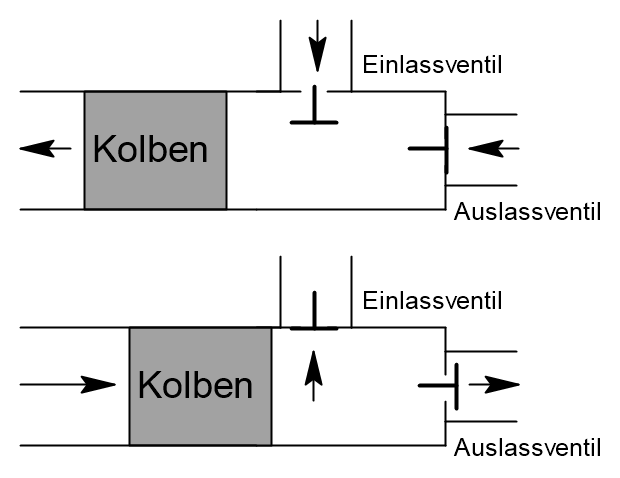
\includegraphics[height=4.25cm]{img/kolbenpumpe}
		\caption{Skizze einer Kolbenpumpe}
		\label{fig:kolbenpumpe}
	\end{minipage}
	%\hspace*{0.05\textwidth}
	\begin{minipage}[b]{0.475\textwidth}
		\centering
		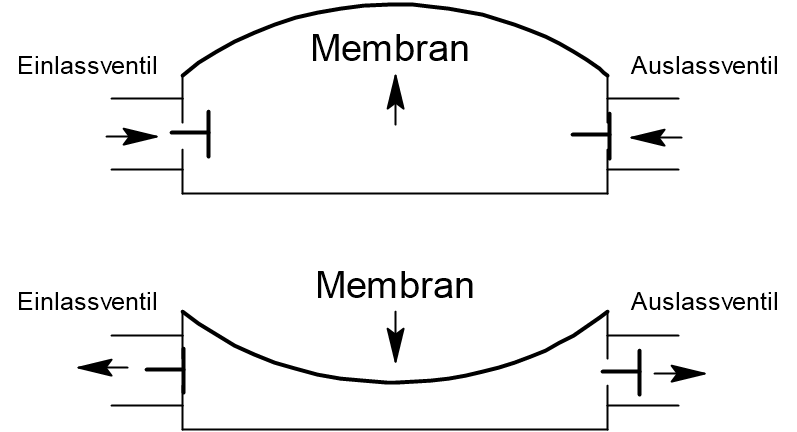
\includegraphics[height=4.25cm]{img/membranpumpe}
		\caption{Skizze einer Membranpumpe}
		\label{fig:membranpumpe}
	\end{minipage}
\end{figure}
\FloatBarrier

Die im Betrieb nutzbaren Stellgrößen bei diesen Pumpen konzentrieren sich aufgrund ihrer Funktionsweise auf die Hublänge und die Hubfrequenz. Durch den geometrisch genau definierten Hubraum und weitestgehend Leckfreien Pumpenventilen und Kolbenabdichtungen, eigenen sich oszillierende Dosierpumpen am günstigsten für die Flüssigkeitsdosierung. Durch das Hubweise fördern der Flüssigkeit ergibt sich jedoch ein digitaler Charakter im Förderstrom. Somit eignen sich diese Pumpen lediglich für diskontinuierliche Dosierung mittels Hubzählung. Der Massenstrom der sich daraus für eine einzylindrige Kolbenpumpe ergibt, ist unter Gleichung \eqref{eq:oz_masse} zu finden. \cite{Vetter.2002}

\begin{equation}
	\label{eq:oz_masse}
	\dot{m} = h_K*A_K*n*\rho*\eta_V
\end{equation}
\begin{parameter}
	\dot{m}		& Fördermassenstrom \\
	h_K			& Hublänge\\
	h_K			& Kolbenquerschnitt\\
	n			& Hubfrequenz\\
	\rho		& Dichte der Flüssigkeit\\
	\eta_V 		& volumetrischer Wirkungsgrad\
\end{parameter}

\paragraph*{Rotierende Verdrängerpumpen} Die Kategorie der rotierenden Dosierpumpen ist im Vergleich zu oszillierenden Dosierpumpen deutlich fassettenreicher. Das hierbei genutzte Verdrängervolumen basiert auf Maßtoleranzen, Spaltmaßen und Elastizitäten des Pumpraumes, welches durch Rotation der Verdrängersystems gefördert wird. Aufgrund dieser Toleranzen treten in rotierenden Verdrängerpumpen für niedrigviskose Flüssigkeiten merkliche, innere Leckagen auf und sind damit weniger genau als oszillierende Verdrängerpumpen. Sie eignen sich daher hauptsächlich für viskose Fluide. Eine Auswahl an typischen, rotierenden Dosierpumpen ist unter Abbildung \ref{fig:rotat_pumpe} dargestellt.

\begin{figure}[h!]
	\centering
	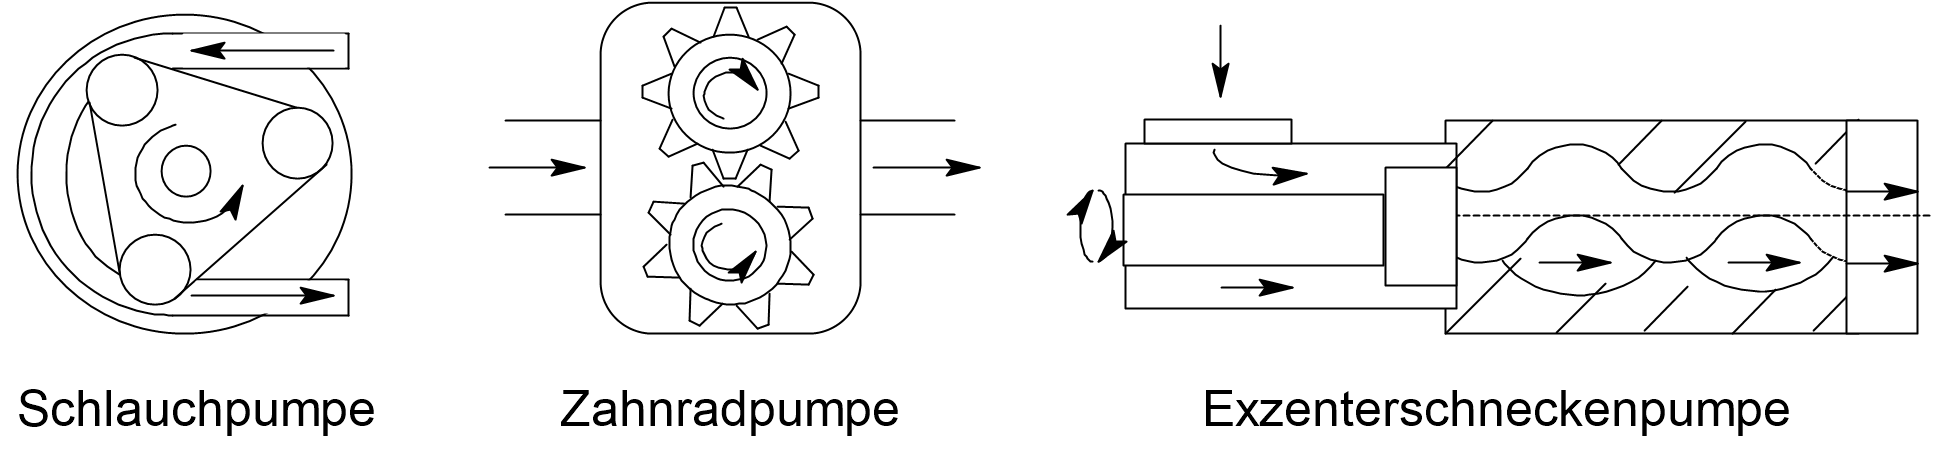
\includegraphics[width=1.0\textwidth]{img/rotationspumpen}
	\caption{Skizzen für Rotationspumpen}
	\label{fig:rotat_pumpe}
\end{figure}
\FloatBarrier

Hauptstellgröße dieser Pumpenart ist die Drehzahl. Ebenso wie bei der Hublänge bzw. der Hubfrequenz oszillierender Verdrängerpumpen besteht bei rotierenden Verdrängerpumpen eine direkte Proportionalität zwischen Drehzahl und Förderstrom. Eine einheitliche Charakteristik des Förderstroms lässt sich für diese Pumpen nicht definieren, da sich trotz Rotationsprinzip die Förderweisen stark unterscheiden. So weisen weißen beispielsweise Schlauchpumpen im Vergleich zu Zahnradpumpen eine viel deutlichere Pulsation des Förderstroms auf, obwohl beide Pumpe den Rotationspumpen zugeordnet werden. Demnach lässt sich auch der Dosierstrom lediglich allgemein wie in Gleichung \eqref{eq:rotations_strom} dargestellt beschreiben. Je nach Pumpentyp lässt sich dann die geometrische Volumenabgrenzung detaillierter ausführen. \cite{Vetter.2002}


\begin{equation}
	\label{eq:rotations_strom}
	\dot{m} = \rho*V_u*n*\eta_V
\end{equation}
\begin{parameter}
	\dot{m}		& Fördermassenstrom \\
	V_u			& Verdrängungsvolumen pro Umdrehung\\
	h_K			& Kolbenquerschnitt\\
	n			& Drehzahl\\
	\rho		& Dichte der Flüssigkeit\\
	\eta_V 		& volumetrischer Wirkungsgrad\
\end{parameter}

Um nach der Vorstellung der verschiedenen Pumpentypen eine Auswahl für die eigene Dosieraufgabe auswählen zu können, sind die verschiedene Kriterien wie Wirkungsgrad, förderbare Viskosität, Druckstabilität, sowie weitere nicht genannte Aspekte heranzuziehen. Einen Überlick hierfür verschafft die Literatur in \mbox{\cite[S. 224 ff.]{Bierwerth.2019}}, sowie ausführlich beschriebene Auswahlhilfen in Form von Tabellen und Diagrammen in \cite[S. 125, 219, 659 ff.]{Vetter.2002}.


\subsubsection{Ermittlung des Dosierstroms}
Je nach Anforderung an die Genauigkeit der Dosierung kommen verschiedene Messsysteme in Frage, um den Dosierstrom zu bestimmen. Hierbei wird zwischen redundanzfreien Dosiersystemen und Dosiersystemen mit Messredundanz unterschieden.\linebreak
Für redundanzfreie Dosiersysteme wird hierbei auf lediglich eine Systemkomponente, wie zum Beispiel der Kennlinie einer Dosierpumpe vertraut, um den geforderten Dosierstrom umzusetzen. Dosiert diese Systemkomponente fehlerhaft bleibt der Fehler unentdeckt. Diese Art der Dosierregelung ist für Prozesse mit geringen Anspruch an Dosiergenauigkeit möglich und deren Konsequenzen im Produktionsprozess tolerierbar sind. In Abbildung \ref{fig:redundanzfrei} ist ein Beispiel für ein redundanzfreies Dosiersystem unter zu Hilfenahme einer Pumpenkennlinie dargestellt.\cite{Vetter.2002}

\begin{figure}[h!]
	\centering
	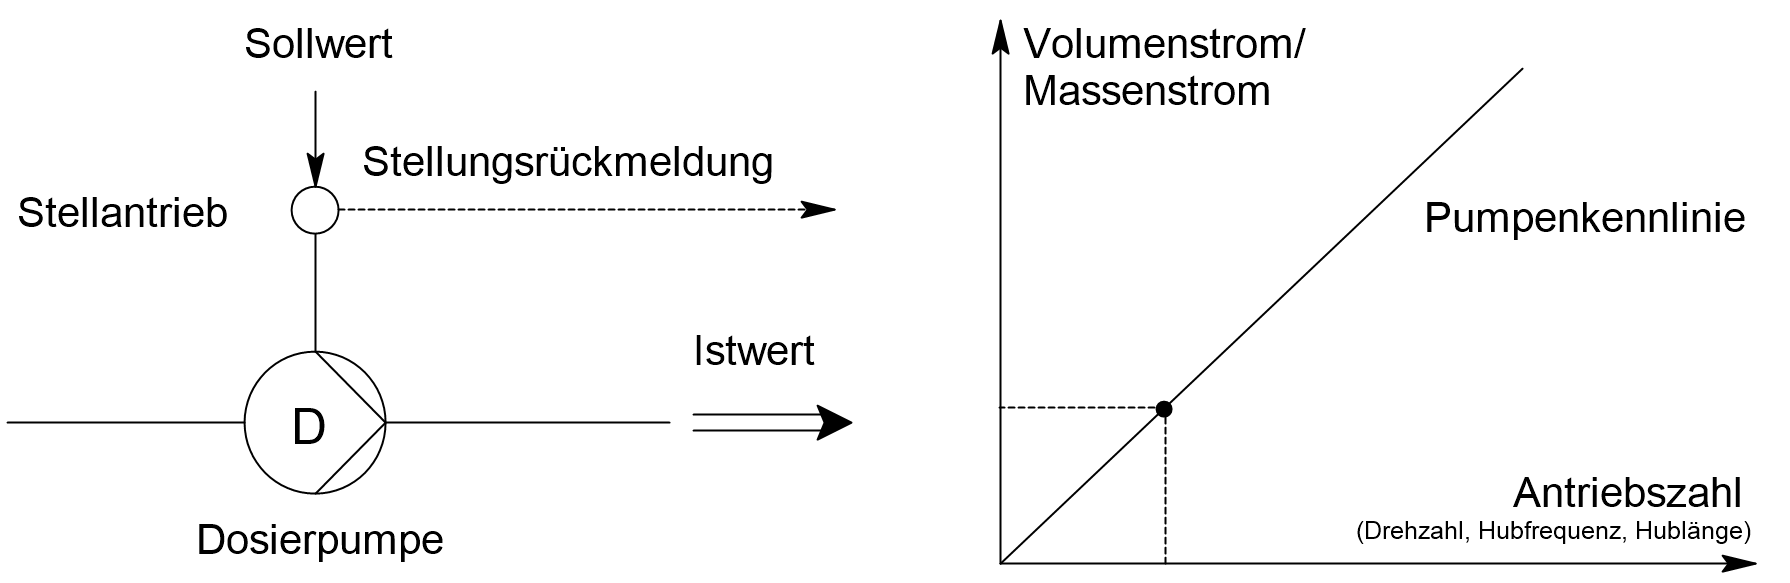
\includegraphics[width=1.0\textwidth]{img/redundanzfrei}
	\caption{Skizze für redundanzfreies Dosiersystem, erstellt nach \cite{Vetter.2002}}
	\label{fig:redundanzfrei}
\end{figure}
\FloatBarrier

In Dosiersystemen mit Messredundanz werden solche Abweichungen durch eine weitere Systemkomponente, wie beispielsweise einem zusätzlichen Durchflussmesser, registriert. Die dadurch geschaffene Fehlervermeidung erhöht die Produktionssicherheit im Prozess, erfordert jedoch auch bereits bei Störung oder Abweichung einer der Komponenten eine Fehlersuche. In Abbildung \ref{fig:redundanz} ist eine beispielhafte Skizze für ein redundant ausgeführtes Dosiersystems mit Dosierpumpe und Durchflussmesser dargestellt.\,\cite{Vetter.2002}

\begin{figure}[h!]
	\centering
	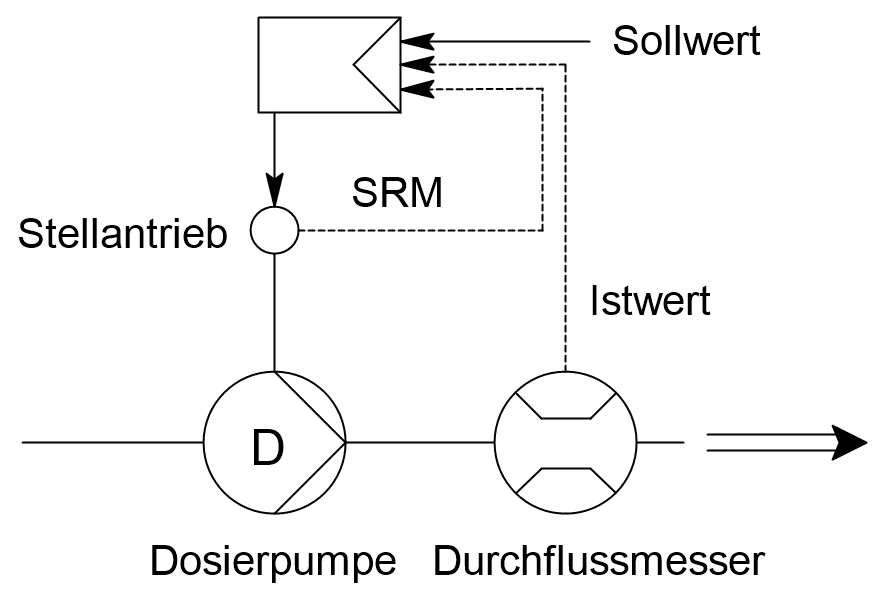
\includegraphics[width=0.5\textwidth]{img/redundanz}
	\caption{Skizze für Dosiersystem mit Redundanz, erstellt nach \cite{Vetter.2002}}
	\label{fig:redundanz}
\end{figure}
\FloatBarrier


Eine Möglichkeit für die redundante Bestimmung des Dosierstroms ist einen Coriolis-Massendurchflussmesser als Systemkomponente zu nutzen. Hierbei wird unter Nutzung einer schwingenden Bewegung, welche auf das strömende Fluid einwirkt, die auftretende Corioliskraft zur Messung des Massenstrom genutzt. Diese wird über induktive Messung der Phasendifferenz zwischen Rohreinlauf und Rohrauslauf bestimmt. Ein Vorteil dieser Art der Durchflussmessung ist, dass neben dem Massenstrom auch Eigenschaften wie die Viskosität, der Massenanteil und die Dichte des Fluides bestimmt werden können. Die Messungen dieser zusätzlichen Parameter basieren dann jedoch auf leicht anderen Messmethoden, als die der Bestimmung des Massenstroms. \cite{Ignatowitz.2015}\linebreak
Nachteil ist jedoch, dass für die Messung nach dem Prinzip der Corioliskraft hohe Strömungsgeschwindigkeiten notwendig sind. Ähnliches gilt übrigens auch für die Messung mittels magnetisch-induktiven Durchflussmesser bei der mindestens ca.\,\SI{0,5}{\meter \per \second} Strömungsgeschwindigkeit notwendig sind. Das kann zum Problem werden, wenn die Strömungsgeschwindigkeit aufgrund von Druckverlusten nicht weiter erhöht werden kann. Das Messverfahren der Ultraschall-Durchflussmessung wäre dann zu den bereits genannten Verfahren eine Alternative, jedoch können durch zu hohe Viskosität des Fluides die erzeugten mechanischen Wellen zu sehr gedämpft werden und es erfolgt keine sinnvolle Messung. \cite{D.Stepanek.Unbekannt, Wikipedia.2021,Wikipedia.2020}\\
Neben den bereits genannten Durchflussmessern gibt es auch so genannte Mengenmesser. Diese beruhen, wenn sie nicht eine Ausführung der zuvor genannten Durchflussmesser sind, meist auf einem Verdrängerprinzip und fungieren als Volumen- oder Geschwindigkeitszähler. Typische Beispiele hierfür sind Ovalradzähler und Turbinenzähler. Speziell Volumenzähler bestimmen die durchgeflossene Menge an Fluid meist durch rotierende Verdrängerkörper wie Zahnräder oder Drehkolben. Durch den Fluss des Fluides drehen sich die Verdrängerkörper und es lassen sich pro Umdrehung die transportierten Volumina des Fluides bestimmen. Vorteil dieser Zähler ist, dass sie meist sehr genau arbeiten und deshalb im Alltag oft als Zähler für Wasser, Benzin  oder Diesel eingesetzt werden. \cite{Ignatowitz.2015}\linebreak
Ihr Nachteil besteht hauptsächlich im mechanischen Wirkprinzip. Dieses hat zur Folge, dass durch zu drehenden Verdrängerkörper für höhere Viskositäten von Fluiden zusätzliche Druckverluste entstehen. Zudem obliegen die Verdrängerkörper durch die mechanische Bewegung oder dem Fluid selbst auch einem gewissen Verschleiß. Zur Bestimmung des Durchflusses ist das gezählte Fördervolumen durch die Förderzeit zusätzlich zu berechnen.\\
Um den Dosierstrom ohne Rohrleitungseinbauten zu bestimmen, ist es möglich ein Loss-in-Weight oder Loss-in-Volume Verfahren zu nutzen. Mit diesen hauptsächlich für schlecht fließende, inhomogene Schüttgüter genutzten Verfahren wird der Massenstrom mittels Differentialdosierer bestimmt. Dieser Differentialdosierer misst den Dosierstrom im klassischen Sinne mit Hilfe einer Waage durch die Gewichtsabnahme über die Zeit. Alternativ ist bei fester, bekannter Geometrie des Dosierbehälters und ausreichender Genauigkeit das selbe Prinzip für eine Füllstands- bzw. Volumenabnahme mit Hilfe eines Radarfüllstandsensors möglich. Vorteil der Förderstrombestimmung über ein solches Loss-in-Weight oder Loss-in-Volume Verfahren liegt darin, dass diese nicht vom Fließverhalten des Mediums beeinflusst werden. Jedoch ist zu bedenken, dass eine ausreichende Auflösung der Messbereiche für die jeweilige Dosierung, sowie der richtige Aufbau für das Messprinzip garantiert werden muss. So ist beispielsweise für die Massenmessung die Entkopplung des Wägesystems und für die Radafüllstandsmessung die einwandfreie Reflexion der Mikrowellensignale an der Dosiergutoberfläche zu gewährleisten. Zudem ist die Dosiergenauigkeit der Radarfüllstandmessung  stark von der Höhe des Dosierbehälters abhängig. Selbst bei $\pm$ \SI{2}{\milli \meter} Messabweichung können diese je nach Behälter bereits mehrere Gramm bis Kilogramm Abweichung bedeuten.\,\cite{Vetter.2002, VEGA.07.02.2022}\linebreak


%%\paragraph*{Radarfüllstandsmessung}
%%\paragraph*{Gravimetrische Erfassung über Wägezellen}
%
%
%\todo[inline]{Beschreibung der Messprinzipien}


%\subsection{Stand der Technik zur Dosierung hochviskoser Verdickungsmittel}

\subsection{Allgemein heuristische Entscheidungsverfahren}
\todo[inline]{Allgemein beschreiben mit verschiedenen Möglichkeiten}

\subsection{Technische Planung}
\subsubsection{R\&I- Fließbild}
\todo[inline]{Erklären was und wofür es das gibt}

\subsubsection{Rohrleitungsplanung}
\todo[inline]{Rohrklassifizierung und Werkstoff Auswahl ??}

\subsubsection{Signalverarbeitungsplanung}
\todo[inline]{Keine Ahnung selber was ausdenken ?}


%\subsection{Normen und Standards}
%
%
%\subsection{Densimeter}
%
%Norm für Viskositätsbestimmung
%
%https://www.din.de/de/neuer-inhalt/wdc-beuth:din21:306904236
%https://www.din.de/de/wdc-beuth:din21:512291
%https://www.din.de/de/neuer-inhalt/wdc-beuth:din21:329765890
%
%\subsection{Wirtschaftliche Aspekte und Entwicklungsperspektiven}

\newpage
\section{Material und Methoden}
\label{sec:durchführung}
%Rahmenbedinungen der Untersuchung
%Auswahl, Einschränkungen und Begründungen
%Erhebungs-, Mess- und Auswertungsverfahren
%Womit und wie haben Sie untersucht ?
\subsection{Allgemein heuristisches Entscheidungsverfahren}
Da es sich diese Bachelorarbeit mit der Findung einer Lösung für eine Problemstellung beschäftigt, wird sich in diesem Abschnitt der Lehre der Heuristik zugewandt. Allgemein beschäftigt sich diese Wissenschaft mit Verfahren um Probleme zu lösen. Im Vordergrund stehen hierbei methodische Anleitungen, Anweisungen und Denkalgorithmen zu schaffen, welche zur Gewinnung neuer Erkenntnisse führen. \cite{Duden.10.02.2022} \linebreak Eine Kategorie dieser Verfahren sind allgemein heuristische Entscheidungsverfahren. Das Wort "`allgemein"' bedeutet in diesem Fall, dass die Methodik des Entscheidungsverfahrens nicht für ein spezielles Entscheidungsproblem konzipiert ist, sondern durchaus für verschiedenste Entscheidungsprobleme nutzbar ist. 
Möglichkeiten, die sich aus der Anwendung eines allgemein heuristischen Verfahrens ergeben sind, dass sie:
\begin{itemize}
	\item zur Lösung beliebiger Entscheidungsprobleme geeignet sind,
	\item die Zielorientierung erhöht wird und damit Fehlentscheidungen vermieden werden und
	\item die Trennung von Faktenwissen und persönlicher Bewertung die Entscheidungsqualität erhöht.
\end{itemize}
Jedoch ergeben sich mit diesen Möglichkeiten auch Grenzen wie zum Beispiel, dass:
\begin{itemize}
	\item allgemein heuristische Entscheidungsverfahren weniger effektiv und effizient sind als ein existierendes spezielles Entscheidungsverfahren,
	\item die Vermeidung von Fehlentscheidungen nicht garantiert werden kann und
	\item mangelndes Fachwissen dadurch nicht kompensiert wird.
\end{itemize}

\subsubsection{Entscheidungsverfahren nach \textsc{Grüning} und \textsc{Kühn}}

Im allgemein heuristischen Entscheidungsverfahren nach \textsc{Grüning} und \textsc{Kühn} beschreiben die Autoren auf welcher Grundlage die Entwicklung ihres Verfahrens beruht. Diese umfasst unter anderem heuristische Prinzipien, Entscheidungsmaximen, Erfahrungen der Autoren als Berater für komplexe Entscheidungssituationen, Erfahrung aus der Entwicklung spezieller heuristischer Entscheidungsverfahren, sowie existierenden allgemein heuristischen Entscheidungsverfahren von anderen Autoren. Mehr dazu, sowie die Beschreibung der Arten von Entscheidungsproblemen findet sich in \cite{Grunig.2013}. Das Verfahren von \textsc{Grüning} und \textsc{Kühn} umfasst dabei sieben Schritte, welche über Schrittsequenzen miteinander verknüpft werden (siehe Abbildung \ref{fig:ahev}).  

\begin{figure}[h!]
	\centering
	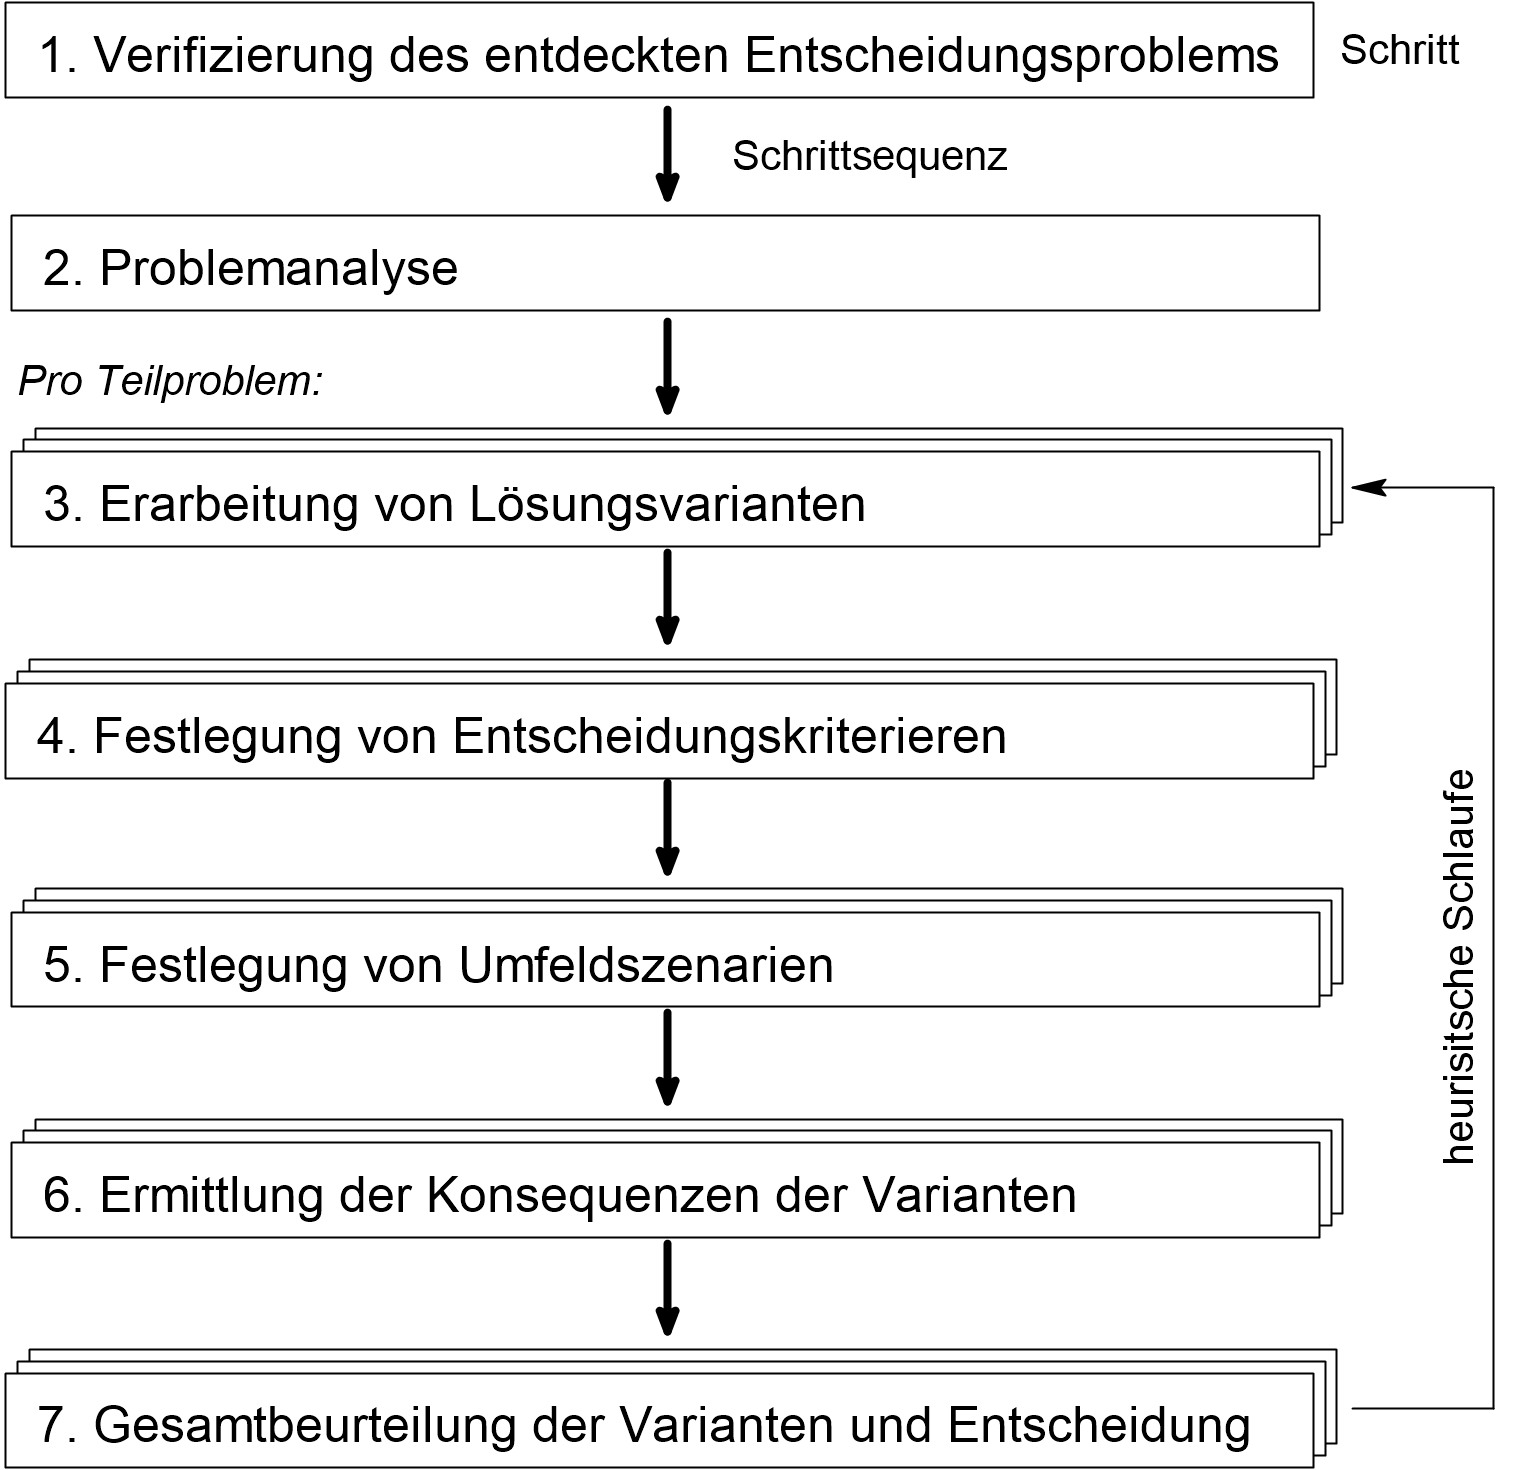
\includegraphics[width=0.5\textwidth]{img/heuristik}
	\caption{Allgemein heuristisches Entscheidungsverfahren, erstellt nach \cite{Grunig.2013}}
	\label{fig:ahev}
\end{figure}
\FloatBarrier

Werden in der Problemanalyse mehrere Teilprobleme festgestellt sind die Schritte\,3 bis 7 für jedes Einzelproblem zu durchlaufen. Die Rückführung, die durch diese Entscheidungsprozesse entsteht wird "`heuristische Schlaufe"' genannt und ist mit dem am häufigsten auftretenden Vertreter in der Entscheidungsfindung in Abbildung \ref{fig:ahev} darstellt. Solche Rückführungen der Entscheidungsschritte können in allen Prozessschritten vorkommen und somit kann es in jeder Teilaktivität zu solch heuristischen Schlaufen kommen. So kann es passieren, dass die Entscheidungskriterien unter Schritt 4 angepasst werden müssen, während bereits in Schritt 6 die Konsequenzen der Lösungsvarianten bestimmt werden. \cite{Grunig.2013} Um das Verfahren anwenden und besser verstehen zu können, werden die einzelnen Schritte des Entscheidungsverfahrens kurzerhand näher erläutert. 
\vspace*{-2.5mm}
\paragraph{Schritt 1: Verifizierung des entdeckten Entscheidungsproblems} In diesem Schritt ist zu prüfen ob die Bearbeitung des Entscheidungsproblems lohnenswert ist und in wie fern sich Soll- und Ist-Zustand voneinander abweichen und auf verlässliche Informationen zurückführen lassen. Lässt sich die Bearbeitung des Problems als lohnenswert und die Beschreibung des Soll- und des Ist-Zustandes auf valide Informationen zurückzuführen ist, gilt das Problem als verifiziert. Je nach Wichtigkeit und Dringlichkeit wird dann festgelegt wer und in welchem Zeitraum an dem Entscheidungsproblem gearbeitet werden soll. Ist keine Aussage zur Wichtigkeit und Dringlichkeit möglich wird von beiden der Worst-Case angenommen.
\vspace*{-2.5mm}
\paragraph{Schritt 2: Problemanalyse} In diesem Schritt wird die Problemstellung abgegrenzt und strukturiert. Im Zuge dieser Analyse erfolgen dann Recherchen und Ermittlungen von relevanten Informationen, um die Problemursachen festzustellen und das Problem in mehrere Teilprobleme zu zerlegen. Danach wird festgelegt welche dieser einzelnen Probleme parallel oder nacheinander bearbeitet werden können. Diese Struktur ist maßgeblich für das Vorgehen in den folgenden Schritten.\\

Die folgenden Schritte 3 bis 7 werden mit jedem Teilproblem einzeln durchgeführt und es kann gegebenenfalls zu heuristischen Schlaufen innerhalb dieser Bearbeitungsschritte kommen. Je nach vorgegebener Struktur unter Schritt 2 kann die Bearbeitung dieser Teilprobleme unterschiedlich angegangen werden.
\vspace*{-2.5mm}
\paragraph{Schritt 3: Erarbeitung von Lösungsvarianten} In diesem Schritt des Entscheidungsverfahrens werden mindestens zwei oder mehr Lösungsvarianten für das Teilproblem erarbeitet. Um den weiteren Bewertungsprozess des Entscheidungsverfahrens rechtfertigen zu können, ist bei der Erarbeitung der Varianten zu beachten, dass sich diese in wesentlichen Merkmalen und nicht nur in Details unterscheiden. 
\vspace*{-2.5mm}
\paragraph{Schritt 4: Festlegung von Entscheidungskriterien} Sind die Lösungsvarianten bestimmt, gilt es sich als nächstes die Entscheidungskriterien festzulegen anhand derer die Varianten evaluiert werden sollen. Die Beschreibung dieser Kriterien besticht dabei durch konkret definierte Maßstäbe anhand derer eine Einschätzung erfolgen kann.
\vspace*{-2.5mm}
\paragraph{Schritt 5: Festlegung von Umfeldszenarien} Dieser optionale Schritt des Entscheidungsprozesses fordert den Aktor der Entscheidung dazu auf, falls nötig, verschiedene Szenarien des Umfeldes zu beschreiben und Eintrittswahrscheinlichkeiten dafür zu definieren. In der Risiko- und Gefahrenanalysen nach dem HAZOP-Verfahren findet eine solche Beurteilung des Umfeldes beispielsweise statt. \todo{Münch nachfragen ob diese Riskotabelle nur für HAZOP galt}
\vspace*{-2.5mm}
\paragraph{Schritt 6: Ermittlung der Konsequenzen der Varianten:} Die zuvor überlegten Entscheidungskriterien und die optionalen Umweltszenarios werden mit den erarbeiteten Lösungsvorschlägen in einer Entscheidungsmatrix zusammengefasst und die sich daraus ergebenen Konsequenzwerte eingetragen. Die Konsequenzwerte werden hierbei durch eingehende Recherchen und dem Wissen und der Erfahrung des Aktors bestimmt und können daher auch einer gewissen Subjektivität unterliegen.
\vspace*{-2.5mm}
\paragraph{Schritt 7: Gesamtbeurteilung der Varianten und Entscheidung} Im letzten Schritt werden die einzelnen Lösungsvarianten in ihrer Gesamtheit beurteilt. Dafür werden irrelevante Varianten eliminiert und danach bestimmt ob für die Wahl der Lösungsvariante ein analytisches oder summarisches Vorgehen bevorzugt wird. Dies entscheidet sich dadurch ob lediglich ein (Einwertigkeit) oder mehrere voneinander unabhängige Entscheidungskriterien (Mehrwertigkeit) die Alternativen unterscheiden und ob es unkontrollierbare Situationen gibt, die für die Variantenwahl entscheidend sind. Im Normalfall kann bei komplexen Problem davon ausgegangen werden, dass diese mehrwertig sind und/oder eine gewisse Unsicherheit oder Ungewissheit der Situation in sich tragen. Laut \cite{Grunig.2013} wird daher ein analytisches Vorgehen bevorzugt bei der Hilfswerte gebildet und verrechnet werden können. Alternativ dazu können sich bei einwertigen und/oder sicheren Entscheidungen auch summarisches Vorgehen eignen, da diese durch Abwägung der Vor- und Nachteile der Varianten weniger komplex und besser interpretierbar sind. 
In der Literatur sind für die jeweiligen Vorgehensweisen verschiedene Methoden, sogenannte Entscheidungsmaximen beschrieben, welche die Überwindung von Mehrwertig, Unsicherheit oder Ungewissheit möglich machen. Eine Möglichkeit der Überwindung der Mehrwertigkeit und der Unsicherheit ist zum Beispiel die auf \textsc{Bernoulli} zurückgehende Maxime des Nutzenerwartungswertes.\linebreak
Ist die Bestimmung der Varianten für die einzelnen Teilprobleme nach analytischen oder summarischen Vorgehen erfolgt, können infolgedessen die vorgeschlagenen Varianten der Teilprobleme mit einander abgestimmt werden. Bildet sich dabei keine heuristische Schleife fällt die Entscheidung über die zu realisierende Variante.

\subsubsection{Nutzenwertmaxime}
Für das analytische Vorgehen bei der Gesamtbeurteilung der Varianten kann die Nutzenwertmaxime zur Überwindung von Mehrwertigkeit genutzt werden. Sie unterscheidet sich von der Maxime des Nutzenerwartungswertes nach \textsc{Bernoulli} durch die fehlende Einbeziehung des Erwartungswertes und überwindet somit auch keine Unsicherheiten. Das muss jedoch bei sicheren Situationen der Entscheidung keinen Nachteil mit sich bringen. Die Entscheidung einer Variante mittels Nutzenwertmaxime umfasst vier Teilaufgaben: 
\vspace*{-2.5mm}
\paragraph{Schritt 1: Umrechnung nicht-numerischer Konsequenzwerte}	\, \\
Nicht-numerische Konsequnzwerte sind anhand einer definierten Skala in Zahlenwerte umzurechnen.
\vspace*{-2.5mm}
\paragraph{Schritt 2: Umrechnung der Konsequenzwerte in Nutzenwerte} \, \\ 
Für jedes Entscheidungskriterium hat die Summe an Nutzwerten der Variante "`1"' zu betragen. Die Nutzwerte der Varianten sind dabei so zu bestimmen, dass die Nutzenwerte zwischen $0$ und 1 liegen und das die günstigste Konsequenz den höchsten Nutzenwert besitzt.
\vspace*{-2.5mm}
\paragraph{Schritt 3: Gewichtung der Entscheidungskriterien} \, \\
Die Summe der Gewichtungen der Entscheidungskriterien sollte auch an dieser Stelle wieder 1 betragen, um eine Vergleichbarkeit zu gewährleisten. Die rein subjektiven Gewichte sollten hierbei die relative Bedeutung für die Zielerreichung widerspiegeln.
\vspace*{-7.5mm}
\paragraph{Schritt 4: Bestimmung der Gesamtkonsequenzen} \, \\
Die Nutzenwerte von jedem Entscheidungskriterium werden mit ihren Gewichten multipliziert und die gewichteten Nutzenwerte pro Entscheidungskriterium addiert. Die Variante mit dem höchsten Nutzenwert entspricht dann dem Entscheidungswert.

\todo[inline]{Vielleicht noch Nutzenwerttabelle zur Veranschaulichung ergänzen ?}

\subsection{Experimentelle Untersuchungen}
Um nähere Erkenntnisse über das Verdickungsmittel zu gewinnen und eine dem Fluid gerechte Auslegung zu gewährleisten  Vorversuche gemacht worden. Hierbei ist zunächst für die strömungstechnische Auslegung die dynamische Viskosität bestimmt worden und infolgedessen untersucht worden welchen Einfluss Verdünnung und Erwärmung auf das Verdickungsmittel haben. Zudem wurden Pumpversuche mit einer Schlauchpumpe durchgeführt, um Erkenntnisse über die Pumpbarkeit zu gewinnen.
\subsubsection{Ermittlung der Viskosität nach DIN EN ISO 2555}
Eine Möglichkeit die dynamische Viskosität einer Dispersion zu bestimmen, ist die Messung mit einem Rotationsviskosimeter nach DIN EN ISO 2555. Da in dieser Norm hauptsächlich ein Rotationsviskosimeter mit Einzelzylinder beschrieben ist, wird an dieser Stelle auf die DIN ISO 3219 verwiesen. In dieser Norm werden zusätzlich Rotationsviskosimeter mit koaxialem Zylinder und Kegel-Platte-Viskosimeter näher beschrieben. \cite{DINDeutschesInstitutfurNormunge.V..Februar2013, DINDeutschesInstitutfurNormunge.V..September2018} \linebreak
Das bei \textsc{Alberdingk Boley Leuna GmbH} verwendete Verfahren zur Viskositätsbestimmung ist angelehnt an die DIN EN ISO 2555 unter Nutzung eines digitalen \textsc{Brookfield}-Rotationsviskosimeters, benannt nach dem Hersteller \textsc{AMETEK$^\text{\textregistered}$\,Brookfield}. Diese Viskosimeter haben den Vorteil preisgünstig zu sein und erlauben ein Messen der Viskosität direkt im Probengefäß. Da jedoch durch das direkte Eintauchen in ein theoretisch beliebiges Probengefäß nur eingeschränkte Übertragbarkeiten und Reproduzierbarkeiten möglich sind, können diese Geräte hauptsächlich für Vergleichsmessungen genutzt werden.  Der Hersteller gibt hierfür an ein \SI{600}{\milli \liter} Becherglas als Probengefäß zu nutzen, jedoch wird in der DIN\,EN\,ISO\,2555 darauf hingewiesen, dass die Becherglasgröße freigewählt werden darf. Für den Vergleich von Messungen rät die Norm dennoch jeweils die gleiche Größe des Becherglases zu nutzen. \cite{ROMPPRedaktion.2008, brookfield_31.01.2022, DINDeutschesInstitutfurNormunge.V..September2018}

%\begin{wrapfigure}{R}{0.33\textwidth}
%	\centering
%	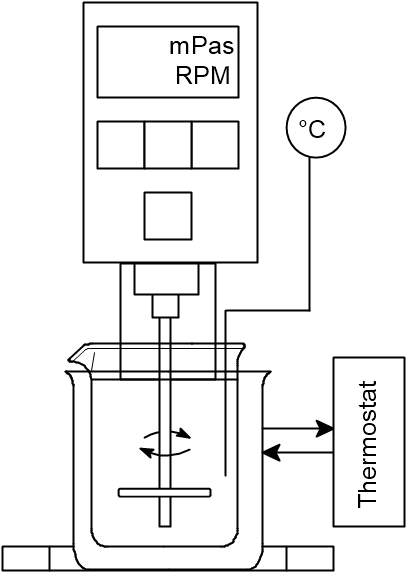
\includegraphics[width=0.25\textwidth]{img/viskosimeter}
%	\caption{Viskositätsmessung mit digitalem \textsc{Brookfield}-\linebreak Rotationsviskosimeter}
%	\label{fig: viskosimeter}
%\end{wrapfigure}
%\FloatBarrier
%%Ende

\begin{figure}[h!]
	\centering
	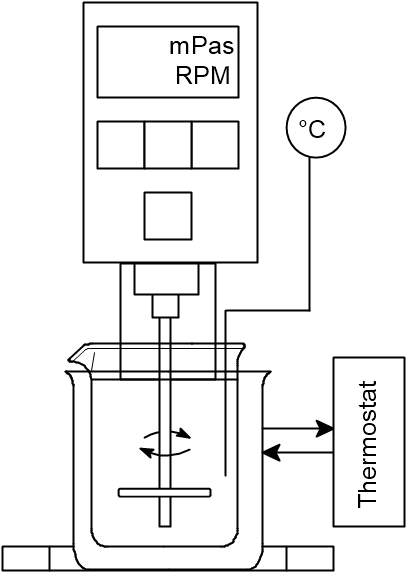
\includegraphics[width=0.25\textwidth]{img/viskosimeter}
	\caption{Viskositätsmessung mit digitalem \textsc{Brookfield}-Rotationsviskosimeter}
	\label{fig: viskosimeter}
\end{figure}
\FloatBarrier
%Ende

Die Messung mittels digitalem \textsc{Brookfield}-Viskosimeter ist vergleichsweise einfach. Benötigt werden hierfür das Viskosimeter in einer Halterung, ein Becherglas, ein Temperaturmessgerät und eine herstellerspezifische Spindel. Soll die Viskosität bei bestimmten Temperaturen, abweichend der Labortemperatur bestimmt werden, ist zusätzlich ein thermostatisches Flüssigkeitsbad nötig (vgl. Abb. \ref{fig: viskosimeter}). Die Messung lässt sich nach dem Aufbau über das Bedienfeld starten in dem Spindel und Drehzahl eingegeben werden. Sobald die Messung startet beginnt sich die Spindel zu drehen.\\
Das Messprinzip eines solchen \textsc{Brookfield}-Viskosimeters basiert auf der Messung der Winkelabweichung, auch Torsion genannt, zwischen der im Viskosimeter verbauten Welle und einer zweiten darunter angeordneten Spindel-Welle mit fest definierten geometrischen Körper. Beide Wellen drehen sich dabei mit der selben Drehzahl  und sind über eine Federeinheit verbunden. Bei Digital-Viskosimetern wird der Messwert der sich dann durch die Winkelabweichung ergibt direkt über ein Display angezeigt.\linebreak
Entscheidend für die Messung der Viskosität ist bei dieser Messmethode die Auswahl des bereits erwähnten Becherglases, sowie der Spindel und der Drehzahl. Spindel und Drehzahl werden dabei unter Einbezug des Viskositätbereiches der Probe nach der gewünschten Präzision und dem Geschwindigkeitgefälle ausgewählt. \cite{DINDeutschesInstitutfurNormunge.V..September2018} 
Durch Tabellen des Herstellers, welche sowohl Spindel als auch Viskositätsbereich in Abhängigkeit von Drehzahl und Gerätekonstanten berechnen lassen, werden diese Entscheidungen vereinfacht. \cite{brookfield_31.01.2022} \linebreak

Um die angegebene Viskosität von ca. \SI{35}{\pascal \second} (vgl. \cite{MunzingChemieGmbH.2020}) zu überprüfen, wurden Untersuchungen zur Viskosität bei \SI{20}{\celsius} durchgeführt. Genutzt wurden dafür ca. \SI{400}{\milli \liter} Verdickungsmittel, die in ein \SI{600}{\milli \liter} Becherglas gefüllt wurden. Gemessen wurden stets mit Spindel 7 des \textsc{Brookfield}-Rotationsviskosimeters für einen Viskositätsbereich von \textcolor{red}{Viskositätsbereich !} bei einer Drehzahl von \SI{50}{\rpm}. Zudem wurde zusätzlich eine Viskositätsmessung mit der gleichen Spindel, bei gleicher Drehzahl und Temperatur für ein \SI{50}{\milli \liter} Becherglas durchgeführt.


\subsubsection{Erwärmungsverhalten}
Im folgenden Abschnitt werden die Untersuchungsmethoden dargelegt, welche den Einfluss die Temperatur auf das Verdickungsmittel TAFIGEL PUR 85 der \textsc{Münzing Chemie GmbH} hat.

\paragraph{Dichte} Um die Dichte in Abhängigkeit von der Temperatur zu bestimmen, wurden entsprechende Daten beim Hersteller angefragt. Eine Rückmeldung über den Dichteverlauf des Verdickungsmittels gab dann aus der Abteilung Forschung und Entwicklung. 

\paragraph{dynamische Viskosität} Die Viskosität in Abhängigkeit von der Temperatur  wurde nach dem ähnlichen Prinzip

\subsubsection{Verdünnungsverhalten}
\subsubsection{Pumpversuche}

\subsection{Recherchearbeit: Literaturarbeit, Fachgespräche und Angebotsanfragen}
\todo[inline]{Vielleicht eher später schreiben ?}

\subsection{Gefährdungsbeurteilung (HAZOP-Verfahren)}
%Nur für die entschiedene Variante

\subsection{Computerunterstützes Zeichnen von Plänen mit AutoCAD}






\newpage
\section{Ergebnisse}
\label{sec:ergebnisse}
%Was waren die Ergebnisse der Untersuchungen?

In diesen Abschnitt werden die Ergebnisse zur Verdickungsmitteldosierung dargestellt. Nach Verifizierung des Problems und dessen Beschreibung erfolgen die Ergebnisse der Untersuchungsmethoden, sowie Entscheidungsverfahren für die Verfahrensplanung und schlussendlich die technische Umsetzung einer Dosiervariante mit einer Gefährdungsbeurteilung.

\subsection{Verifizierung und Analyse des Dosierproblems}
Im ersten Schritt wurde der Ist-Zustand der Dosierung erfasst, sowie die Gegebenheiten im Werk analysiert. Danach erfolgte das Zusammentragen der Anforderungen an eine halbautomatisch umgesetzte Dosierung.
 
\subsubsection{Ist-Zustand: Produktionsweise und aktuelles Dosierverfahren}
Das herzustellende Produkt für das eine halbautomatische Verdickerdosierung umgesetzt werden soll nennt sich \textit{AC 548}. Es ist eine Acrylat-Copolymer Dispersion und kann als Betonschutz, Fassadenfarben, wärmeaktivierbare Klebstoffe, Putze und Buntsteinputze verwendet werden. Produziert wird \textit{AC 548} im Batch-Betrieb à \SI{14}{\tonne} und die Planung erfolgt vorzugsweise in Kampagnen. \cite{ALBO.22.02.2022} \linebreak
Derzeit wird für dieses Produkt das Verdickungsmittel Rheobyk-H 3300 VF der \textsc{Byk-Chemie GmbH} eingesetzt, welches jedoch im Laufe des Jahres 2022 durch Einstellen der Produktion mit dem Verdickungsmittel TAFIGEL PUR 85 der \textsc{Münzing Chemie GmbH} substituiert werden soll. Die aktuelle Dosierung beläuft sich dabei auf die Nutzung eines \SI{0}{\liter}-Kunststofffasses als Dosierbehälter. Hierfür werden zunächst \SI{22}{\kilo \gram} des Verdickungsmittels in einem "`Transportfass"' im Chemikalienlager abgewogen und dann am entsprechenden Einstelltank bereit gestellt. Für den Start der Dosierung wird das "`Dosierfass"', welches mit einem Dosierloch an der Fassunterseite versehen ist, in das Fallschutzgitter des Mannlochs gehängt und der Inhalt des Transportfasses in das Dosierfass gekippt. Schematisch dargestellt ist diese Dosierung in Abbildung \ref{fig:aktuelle_dosierung}.

\begin{figure}[h!]
	\centering
	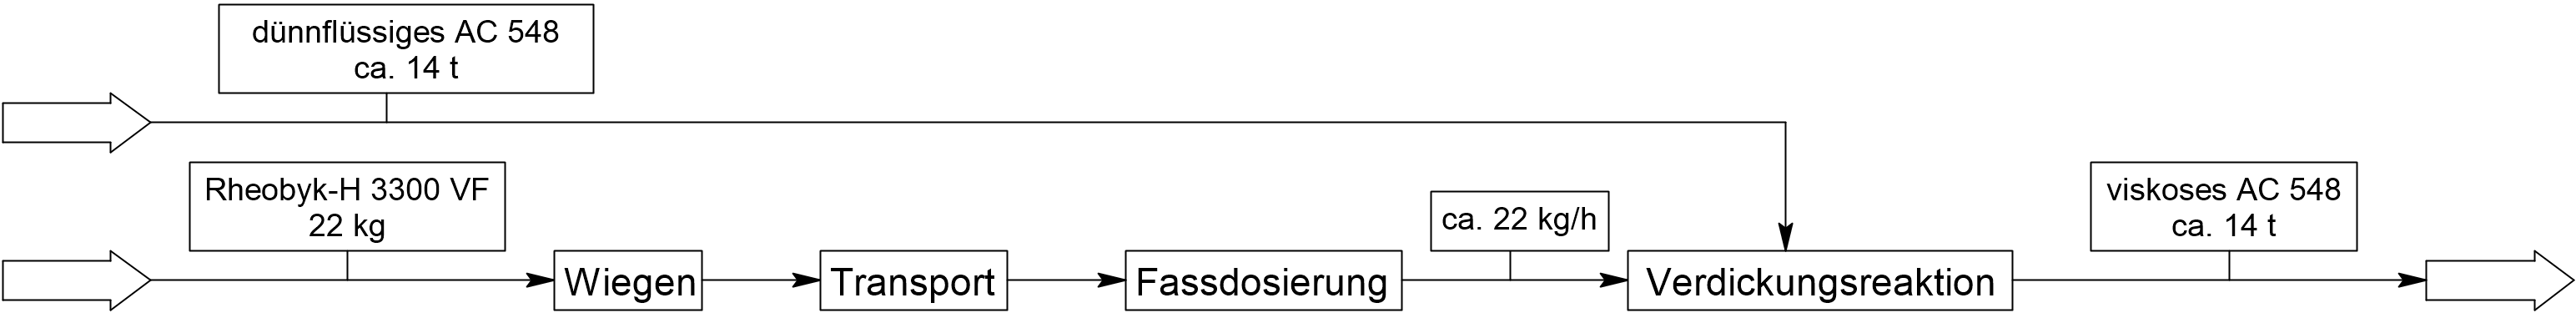
\includegraphics[width=\textwidth]{img/aktuelle_dosierung}
	\caption{Aktuelle Dosierung des Verdickungsmittels Rheobyk-H 3300 VF}
	\label{fig:aktuelle_dosierung}
\end{figure}
\FloatBarrier
%Ende

Vorteile dieses Dosierverfahrens sind die einfache und kostengünstige Umsetzung. Dem entgegen steht jedoch, dass neben dem "`Dosierloch"' und dem Fass selbst keine Einstellparameter vorhanden sind und der Dosierstrom weder messtechnisch erfasst noch im Prozessleitsystem (PLS) einsehbar ist. Zudem kann die Umsetzung für die Dosierung nur bedingt hygienisch erfolgen wie unter anderem in Abbildung \ref{fig:dosierfass} zu erkennen ist.

\begin{figure}[h!]
	\centering
	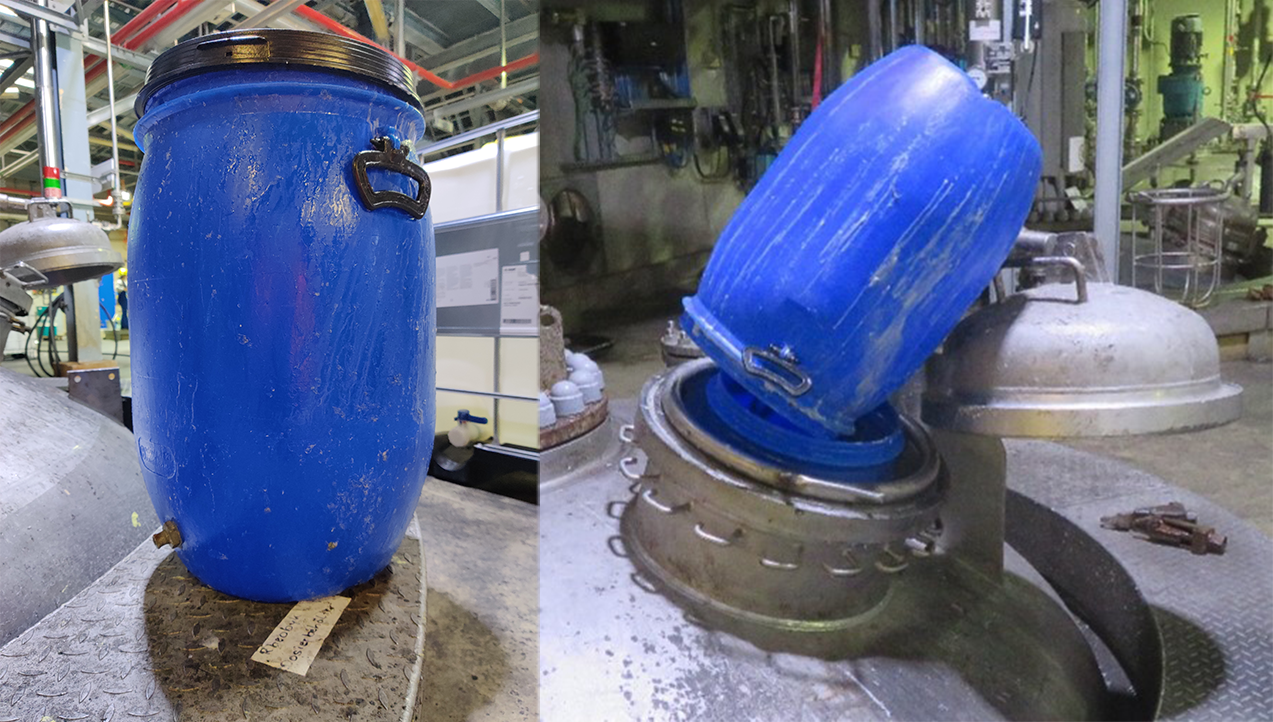
\includegraphics[width=0.5\textwidth]{img/dosierfass}
	\caption{Fotografien des Dosier- und des Transportfasses}
	\label{fig:dosierfass}
\end{figure}
\FloatBarrier
%Ende

\subsubsection{Soll-Zustand: Anforderung an die Dosierung}
Die Anforderungen an eine automatisierte Dosierung gliedern sich in mehrere Interessensgruppen auf. Beginnend mit der \textit{Technik}, sollen unter diesem Begriff jegliche Anforderungen der Prozess- und Sicherheitstechnik beschrieben sein. Beispielsweise fallen darunter die Dosierrate, die Dosiergenauigkeit und der zu beachtende Ex-Schutz. Die zweite Gruppierung beschreibt die Anforderungen der \textit{Produktion}, sprich die Interessen der auszuführenden Chemiefacharbeiter in der Anlage. Eine Forderung stellt dabei die einfache Bedienbarkeit dar. Zuletzt soll jedoch auch die \textit{Wartung} entsprechend leichtgängig und der Verschleiß des Dosiersystems gering sein. Die Forderungen aus den verschiedenen Perspektiven sind in Tabelle \ref{tab:anforderungen} zusammenfasst und wurden durch erfragen des Personals ermittelt und durch vorgegebenen Prozessparametern festgelegt.

% Table generated by Excel2LaTeX from sheet 'Daten'
\begin{table}[h!]
	\renewcommand*{\arraystretch}{1.2}
	\centering
	\caption{Anforderungen an die Verdickungsmittel-Dosierung}
	\label{tab:anforderungen}
	\resizebox{\textwidth}{!}{
		\begin{tabulary}{1.2\textwidth}{LL|L|L}
			\hline
			\multicolumn{2}{l|}{\textbf{Technik}} & \textbf{Produktion} & \textbf{Wartung}\\
			\hline
			Dosierrate: & 22 bis \SI{44}{\kilo \gram \per \hour}&einfache Bedienbarkeit&geringer Verschleiß\\
			Dosiergenauigkeit: & $\pm \, \SI{200}{\gram}$	& leichte Reinigung & leichte Wartung\\
			Ex-Schutz:	 & Zone 2 &Zeitersparnis&\\
			Risiko:  &minimal&&\\
			Verdickungsmittel: &TAFIGEL PUR 85&&\\
			Prozessleitsystem: &im PLS einsehbar&&\\
			Adaptierbarkeit:& für weitere Tanks adaptierbar &&\\
			Aufstellungsort: &siehe Abbildung \ref{fig:aufstellungsort}&&\\
			Einleitung: &siehe Abbildung \ref{fig:flansch}&&\\
			\hline
	\end{tabulary}}
\end{table}%
\FloatBarrier

Da weder die geforderte Dosiergenauigkeit erfasst, noch der Dosierstrom in der aktuellen Dosierung gemessen wird, ist eine signifikante Differenz zwischen Ist- und Soll-Anforderung an die Dosierung aus Perspektive der Technik erfüllt und das Dosierproblem somit als solches verifiziert. Die Perspektive der Produktion unterstützt diese Verifikation, da Anforderungen aufgrund der benötigten Vorbereitungszeit und der Sauberkeit der Dosierprozesses derzeit nicht erfüllt werden. Aus Sicht der Wartung besteht kein Handlungsbedarf.

\begin{figure}[h!]
	\begin{minipage}[b]{0.475\textwidth}
		\centering
		\includegraphics[height=4.25cm]{img/aufstellungsort}
		\caption{Aufstellungsort für Dosierung}
		\label{fig:aufstellungsort}
	\end{minipage}
	%\hspace*{0.05\textwidth}
	\begin{minipage}[b]{0.475\textwidth}
		\centering
		\includegraphics[height=4.25cm]{img/flansch}
		\caption{Flansch für eingehenden Dosierstrom}
		\label{fig:flansch}
	\end{minipage}
\end{figure}
\FloatBarrier

%geringer Verschleiß
%leichte Wartung
%einfach zu Bedienen
%leichte Reinigung --> Spülbarkeit
%Dosiergenauigkeit und DOsierstrom
%--> SAmmeln von Informationen im Werk
% Platz im Werk mit Geometrie
%
%Kampagne
%Mitarbeiterkosten sparen
%Zeitersparnis
%Einfachheit
%Ex-Schutz
%PLS
%Prozesssicherheit

\subsubsection{Ergebnisse der experimentellen Untersuchungen}
In der zu planenden Dosierung soll auf das Verdickungsmittel TAFIGEL PUR 85 der \mbox{\textsc{Münzing Chemie Gmbh}} zurückgegriffen werden. Laut Hersteller handelt es sich hierbei um einen assoziativen Polyurethan-Verdicker, welcher durch Gerüstbildung zwischen Verdickermolekülen, Bindemittel und Pigmentpartikeln die gewünschte Viskosität hervorruft und stabilisiert. Diese Beschreibung deckt sich mit der unter Abschnitt \ref{sec:grundlagen} formulierten Beschreibung der Assoziativverdicker. \cite{MunzingChemieGmbH.2014}
%--> Datenblätter
Die Ergebnisse der Viskositätsmessungen gliedern sich nach der Durchführung in Abschnitt \ref{sec:durchführung} in die Verifizierung der angegebenen Viskosität, der Untersuchung der Temperaturabhängigkeit, der Untersuchung der Verdünnungsabhängigkeit und in Pumpversuche.
Beginnend mit der Verifizierung der angegeben Viskosität sind in Abbildung \ref{dia:visko} die gemessenen Viskositäten des TAFIGEL PUR 85 und des Rheobyk-H 3300 VF dargestellt. 

%START DIAGRAMM

\begin{figure}[h]
	\begin{center}
		%\resizebox{\textwidth}{!}{
		\begin{tikzpicture}
			\begin{axis}[
				grid=both,
				grid style={line width=.1pt, draw=gray!10},
				major grid style={line width=.2pt,draw=gray!50},
				width= 0.95 \textwidth,
				height=0.5\textwidth,
				symbolic x coords={, Messreihe 1, Messreihe 2, Messreihe 3, Messreihe 4, Messreihe 5, \shortstack[c]{\SI{50}{\milli \liter} \\ Becherglas},},
				axis y line = left,
				axis x line = bottom,
				xtick=data,
				ytick={0,5,...,65},
				ymax = 65,
				ymin=0,
				ylabel=dynamische Viskosität in \si{\pascal \second},
				legend style={at={(0.475,1.05)},anchor=west},
				legend cell align={left}]
				%Tafigel
				\addplot[color=black,mark=*, only marks] coordinates {
					(Messreihe 1, 49.080)
					(Messreihe 2, 50.760)
					(Messreihe 3, 52.000)
					(Messreihe 4, 53.000)
					(Messreihe 5, 51.600)
					(\shortstack[c]{\SI{50}{\milli \liter} \\ Becherglas}, 50.87)
				};
				\addplot[color=black,dashed] coordinates {
				(Messreihe 1, 51.21)
				(\shortstack[c]{\SI{50}{\milli \liter} \\ Becherglas}, 51.21)
				};
				%Rheobyk
				\addplot[color=black,mark=o, only marks] coordinates {
					(Messreihe 1, 24.000)
					(Messreihe 2, 24.800)
					(Messreihe 3, 22.880)
					(Messreihe 4, 23.890)
					(Messreihe 5, 24.200)
					(\shortstack[c]{\SI{50}{\milli \liter} \\ Becherglas}, 23.32)
				};
				\addplot[color=black,dotted] coordinates {
					(Messreihe 1, 23.85)
					(\shortstack[c]{\SI{50}{\milli \liter} \\ Becherglas}, 23.85)
				};
			\legend{Viskosität - TAFIGEL PUR 85, Mittelwert (\SI{51}{\pascal \second}), Viskosität - Rheobyk-H 3300 VF, Mittelwert (\SI{24}{\pascal \second}) };
			\end{axis}
		\end{tikzpicture}
		%}
		\caption{Dynamische Viskositäten der Verdickungsmittel TAFIGEL PUR 85 und Rheobyk-H 3300 VF}
		\label{dia:visko}
	\end{center}
\end{figure} 

\FloatBarrier 
%ENDE

Die sich aus den Messwerten ergebenden Mittelwerte ergeben eine Viskosität für TAFIGEL PUR 85 mit \SI{51}{\pascal \second} und für Rheobyk-H 3300 VF \SI{24}{\pascal \second}. Zum Vergleich: Die Viskosität des TAFIGEL PUR 85 ist im Sicherheitsdatenblatt mit rund \SI{35}{\pascal \second}  angegeben. Auf Nachfrage beim Hersteller ist diese Schwankung produktionsbedingt und beeinträchtigt die Wirksamkeit des Verdickungsmittels nicht. \cite{MunzingChemieGmbH.2020} Ebenfalls zu erkennen ist, dass die Messwerte Abweichungen vom Mittelwert aufzeigen. Statistisch ergeben sich daraus relativen Standardabweichungen für die Messwerte des TAFIGEL PUR\,85 mit \SI{2,4}{\percent} und für das Rheobyk-H 3300 VF mit \SI{2,6}{\percent}. Die Messungen im \SI{50}{\milli \liter}, statt im \SI{600}{\milli \liter} Becherglas zeigten keine maßgeblichen Unterscheide.\linebreak
%--> nach DIN
%--> beide Verdickungsmittel
Eine weitere Untersuchung beschäftigte sich mit der Temperaturabhängigkeit des Verdickungsmittels. Dafür wurde zum einen der Verlauf der Dichte in Abhängigkeit von der Temperatur für das TAFIGEL PUR 85 bei der \textsc{Münzing Chemie GmbH} angefragt. Die erhaltenen Daten sind in Abbildung \ref{dia:dichte} zu sehen.

%START DIAGRAMM

\begin{figure}[h]
	\begin{center}
		%\resizebox{\textwidth}{!}{
			\begin{tikzpicture}
				\begin{axis}[
					grid=both,
					grid style={line width=.1pt, draw=gray!10},
					major grid style={line width=.2pt,draw=gray!50},
					width= 0.95 \textwidth,
					height=0.33\textwidth,
					%symbolic x coords={, Messreihe 1, Messreihe 2, Messreihe 3, Messreihe 4, Messreihe 5, \shortstack[c]{\SI{50}{\milli \liter} \\ Becherglas},},
					axis y line = left,
					axis x line = bottom,
					xtick={0,5,...,50},
					ytick={950,975,...,1050},
					xmax=50,
					ymax = 1050,
					ymin=950,
					xmin=0,
					ylabel=Dichte in \si{\kilo \gram \per \kmeter},
					xlabel = Temperatur in \si{\celsius},
					legend style={at={(1.0,0.95)},anchor=east},
					legend cell align={left},
					ylabel style={yshift=0.4cm},]
					%Tafigel
					\addplot[color=black,mark=*, only marks] coordinates {
						(10, 1034)
						(20, 1010)
						(30, 1008)
						(40, 1001)
					};				
					\legend{Dichte - TAFIGEL PUR 85};
				\end{axis}
			\end{tikzpicture}
			%}
		\caption{Dichte des TAFIGEL PUR 85 in Abhängigkeit von der Temperatur}
		\label{dia:dichte}
	\end{center}
\end{figure} 

\FloatBarrier 
%ENDE

Zu erkennen ist, dass sich die Dichte im Bereich zwischen 10 und \SI{40}{\celsius} mit steigender Temperatur verringert. Der Verlauf und der Umfang der Daten lässt nicht eindeutig auf einen linearen Zusammenhang zwischen Dichte und Temperatur schließen, jedoch ist erkennbar, dass ein signifikanter Unterschied in der Dichte für 10 und für \SI{40}{\celsius} besteht. Im Bereich zwischen 20 und \SI{30}{\celsius} bleibt die Dichte hingegen konstant. Aus den Daten wurde ermittelt, dass zwischen den Messungen eine relative Standardabweichung von \SI{1,4}{\percent} vorliegt.\linebreak
Neben dem Erfragen des Zusammenhangs zwischen Dichte und Temperatur ist auch die Abhängigkeit der Viskosität von der Temperatur untersucht worden. Der Grund hierfür liegt in der zuvor bestimmten Viskosität des Verdickungsmittels bei rund \SI{50}{\pascal \second}. Da im Regelfall bei der \textsc{Alberdingk Boley Leuna GmbH} keine so hohen Viskositäten gefördert werden, bot sich die Überlegung an die Viskosität durch Wärmezufuhr zu reduzieren. Das Ergebnis der dafür genutzten Versuchsreihe ist in Abbildung \ref{dia:temp} zu finden. Darin lässt sich erkennen, dass der Zusammenhang zwischen Viskosität und Dichte in diesem Temperaturbereich eine Linearität mit einem Bestimmtheitsmaß von \SI{99,6}{\percent} aufweist. Mit steigender Temperatur sinkt dabei die Viskosität. Der negative Anstieg lässt zudem darauf deuten, dass bei einer Temperaturerhöhung um \SI{5}{\kelvin} eine Verringerung der Viskosität um \SI{10}{\pascal \second} stattfindet.

%START DIAGRAMM

\begin{figure}[h]
	\begin{center}
		%\resizebox{\textwidth}{!}{
			\begin{tikzpicture}
				\begin{axis}[
					grid=both,
					grid style={line width=.1pt, draw=gray!10},
					major grid style={line width=.2pt,draw=gray!50},
					width= 0.95 \textwidth,
					height=0.4\textwidth,
					%symbolic x coords={, Messreihe 1, Messreihe 2, Messreihe 3, Messreihe 4, Messreihe 5, \shortstack[c]{\SI{50}{\milli \liter} \\ Becherglas},},
					axis y line = left,
					axis x line = bottom,
					xtick={0,5,...,50},
					ytick={0,5,...,65},
					xmax=50,
					ymax = 65,
					ymin=0,
					xmin=0,
					ylabel=dynamische Viskosität in \si{\pascal \second},
					xlabel = Temperatur in \si{\celsius},
					legend style={at={(1.,1.125)},anchor=east},
					legend cell align={left},
					%ylabel style={yshift=0.4cm},
					]
					%Tafigel
					\addplot[color=black,mark=*, only marks] coordinates {
						(21, 50.1)
						(25, 39.5)
						(30, 30.2)
						(35, 19.2)
						(39, 12.6)
					};
				
				\addplot [domain = 0:50, dashed] {-2.07*x+92.26};
							
					\legend{Viskosität - TAFIGEL PUR 85,$\eta(\vartheta) = -\SI{2,07}{\pascal \second \per \celsius}*\vartheta+\SI{92,26}{\pascal\second} \, | \, R^2 = \SI{99,6}{\percent}$};
				\end{axis}
			\end{tikzpicture}
			%}
		\caption{Dynamische Viskosität des TAFIGEL PUR 85 in Abhängigkeit von der Temperatur}
		\label{dia:temp}
	\end{center}
\end{figure} 
\FloatBarrier 
%ENDE
Zusätzlich wurde neben dem Aspekt der Erwärmung des Verdickungsmittels wurde auch der Effekt der Verdünnung auf die Viskosität untersucht. Es wird erwartet, dass mit sinkender Konzentration an Verdickungsmittel die Viskosität des Verdickungsmittels ebenfalls sinkt. In Abbildung \ref{dia:verdunnung} sind die Messergebnisse der Viskositäten beider Verdickungsmittel TAFIGEL PUR 85 und Rheobyk-H 3300 VF dargestellt. In separaten x-Achsen sind der Anteil an Verdickungsmittel und der Anteil an reiner Aktivsubstanz der Verdickungsmittels aufgetragen.

%START DIAGRAMM

\begin{figure}[h]
	\begin{center}
		%\resizebox{\textwidth}{!}{
			\begin{tikzpicture}
				\begin{axis}[
					grid=both,
					grid style={line width=.1pt, draw=gray!10},
					major grid style={line width=.2pt,draw=gray!50},
					width= 0.95 \textwidth,
					height=0.4\textwidth,
					%symbolic x coords={, Messreihe 1, Messreihe 2, Messreihe 3, Messreihe 4, Messreihe 5, \shortstack[c]{\SI{50}{\milli \liter} \\ Becherglas},},
					axis y line = left,
					axis x line = bottom,
					xtick={0,10,...,100},
					ytick={0,5,...,65},
					xmax=100,
					ymax = 65,
					ymin=0,
					xmin=0,
					ylabel=dynamische Viskosität in \si{\pascal \second},
					xlabel = Verdickermassenanteil in \si{\mpercent},
					legend style={at={(0.025,0.8)},anchor=west},
					legend cell align={left},
					%ylabel style={yshift=0.4cm},
					]
					%Tafigel
					\addplot[color=black,mark=*, only marks] coordinates {
						(20, .230)
						(30, .800)
						(40, 1.700)
						(50, 4.500)
						(60, 6.650)
						(71, 13.650)
						(79, 21.240)
						(84, 25.650)
						(100, 49.300)
					};
				%Rheobyk
				\addplot[color=black,mark=o, only marks] coordinates {
					(10, 0.300)
					(20, 2.400)
					(30, 3.870)
					(41, 5.400)
					(48, 6.600)
					(57, 6.600)
					(81, 5.000)
					(100, 4.700)
	
				};
					\legend{Viskosität - TAFIGEL PUR 85, Viskosität - Rheobyk-H 3300 VF};
				\end{axis}
			\begin{axis}[
				width= 0.95 \textwidth,
				height=0.4\textwidth,
				%symbolic x coords={, Messreihe 1, Messreihe 2, Messreihe 3, Messreihe 4, Messreihe 5, \shortstack[c]{\SI{50}{\milli \liter} \\ Becherglas},},
				hide y axis,
				axis x line = top,
				xtick={0,2.5,...,25},
				xmax=25,
				xmin=0,
				xlabel = Aktivsubstanz in \si{\mpercent},
				legend style={at={(1.,1.125)},anchor=east},
				legend cell align={left},
				]
				%Tafigel
				\addplot[draw=none, forget plot] coordinates {
					(5, .230)
					(7.5, .800)
					(10, 1.700)
					(12.5, 4.500)
					(15, 6.650)
					(17.7, 13.650)
					(19.9, 21.240)
					(20.9, 25.650)
					(25, 49.300)
				};
			\end{axis}
			\end{tikzpicture}
			%}
		\caption{Dynamische Viskositäten der Verdickungsmittel  TAFIGEL PUR 85 und Rheobyk-H 3300 VF in Abhängigkeit vom Massenanteil des Verdickungsmittels bzw. dem Anteil an Aktivsubstanz}
		\label{dia:verdunnung}
	\end{center}
\end{figure} 
\FloatBarrier 
%ENDE
Durch dieses Diagramm zeigt sich, dass sich beide Verdickungsmittel in ihrem Verdünnungsverhalten deutlich unterscheiden. Während das Rheobyk-H 3300 VF ab \SI{40}{\mpercent} eine vergleichsweise stabile Viskosität in Abhängigkeit von der Verdünnung aufzeigt, lässt sich für das TAFIGEL PUR 85 eine starke Abhängigkeit zwischen Viskosität und Verdickermassenanteil festzustellen. Auffallend ist zudem, dass die Viskosität des Rheobyk-H 3300 VF im Bereich zwischen 50 und \SI{60}{\mpercent} höher ist als mit einem Verdickeranteil von \SI{100}{\mpercent}.
%
%\subsubsection{Verdünnungsverhalten}
%%--> Eigenregie
%
%\subsubsection{Erwärmungsverhalten}
%%--> beim Hersteller angefragt
%
Im Laufe der Überlegungen zur Umsetzung der Dosierung wurde die Möglichkeit der Dosierung mit einer Pumpe in Betracht gezogen. Durch die hohen Viskosität und den Anforderungen an Sauberkeit und Wartung, sollte zunächst die Pumpbarkeit des TAFIGEL PUR 85 mit einer Schlauchpumpe überprüft werden. Die Ergebnisse der Massenströme bei verschiedenen Drehzahlen ist im Diagramm unter Abbildung \ref{dia:pumpe} gezeigt.



\subsubsection*{Pumpversuche}

erster Volumenstrom erst nach einer Stunde zu erkennen 


\todo[inline]{Entscheidungsprobleme werden aufgrund des Umfangs und der schweren Nachvollziehbarkeit nicht dargestellt}

\subsection{Entscheidungsprobleme}
\label{subsec:entscheidungsprobleme}
\subsubsection{Entscheidung für ein Verfahren}
%Verdünnen
%spülen
%erwrämen
%nichts 
%Rühren
%kombinationen
%aktuelles Verfahren

\subsubsection{Entscheidung für Gebindetyp}
%Preis nachfrage
%\subsubsection{Angebotsanfrage}
%\subsubsection{Entscheidungsverfahren}

\subsubsection{Entscheidung für Pumpendosierung oder Dosierbehälter}

\subsubsection{Auswahl des Pumpentyps}
%\subsubsection{Literaturarbeit}
%Bücher gelesen für Auswahlhilfe
%\subsubsection{Fachgespräche und Angebotsanfrage}
%\subsubsection{Entscheidungsverfahren}

%\subsection{Auswahl des Pumpentyps, sowie des Leitungsdurchmessers}
%Gespräche geführt und Leitung hat sich nach möglichen Drücken in der Anlage und Pumpentyp, sowie Berechnungen gerichtet gerichtet

\subsubsection{Auswahl des Messverfahrens}

\subsection{Technische Planung für Verdickungsmitteldosierung}
\subsubsection{Verfahrensfließbild der Verdickerdosierung}
\subsubsection{R\&I- Fließbild der Verdickerdosierung}
\subsubsection{Rohrleitungsplanung der Verdickerdosierung}
%vertretbarer Druckverlust
%Rohrdurchmesser und Nenndruck
%--> Rohrleitungsklassifizierung

\subsubsection{EMSR-Plan der Messtechnik für die Dosierung}

\subsection{Gefährdungsbeurteilung der geplanten Verdickungsmitteldosierung}



\section{Diskussion}
\label{sec:diskussion}
%Bewertung hinsichtlich:
%zentraler Aufgabe
%wissenschaftlicher, technischer Kontext
%Verallgemeinbarkeit
%persönliche Schlussfolgerungen

\subsection{Diskussion der experimentellen Untersuchungen}

\subsection{Diskussion der Entscheidungen}

\subsection{Diskussion der Rohrleitungsplanung}

\subsection{Diskussion der Gefährdungsbeurteilung}

Viskositätsmessung nach DIN EN ISO 2555, statt DIN EN ISO 3219 --> laut DIN EN ISO 2555 macht das Messverfahren für newtonsches Fluid keinen Unterschied

Trockenschrank könnte Lösungsmittel entfernen --> nicht signfikant --> dennoch geringere Viskosität durch Erwärmung

Becherglas 50 ml bei Verdünnungsmessung --> Anhaltspunkt für verlauf --> reicht für weitere Auswertung, da ungefähr selbes ergebnis bei 600 ml Becherglas

--> Dichte Somit könnten im betrachteten Temperaturbereich bereits Schwankungen von \SI{5}{\kelvin} einen registrierbaren Einfluss auf die Genauigkeit einer rein volumetrischen Dosierung haben.

Vergleich der Viskositäten in der Disskussion

\section{Zusammenfassung und Schlussfolgerungen}
\label{sec:zusammenfassung}
%Ergebnisgewinn
%HAndlungsempfhelung für die Praxis
%Ausblick auf künftige Entwicklungen, Notwendigkeiten, Folgeprojekte

%\section{Fehlerbetrachtung}
\label{sec:fehler}


%%Praktikumsskript, Modul ………, Versuch …….., Prof. Musterprof. 
%%DIN 12345, Jahr der Veröffentlichung 
%%Link der Internetseite, Zugriffsdatum 
%%Buchtitel, Autor, Verlag, Veröffentlichungsjahr 
%
%Literaturverzeichnis Bücher
\bibliography{Literatur2}
\bibliographystyle{alphadin}
\addcontentsline{toc}{section}{Literaturverzeichnis}


%Verzeichnis aller Bilder
\label{sec:bilder}
\listoffigures
\addcontentsline{toc}{section}{Abbildungsverzeichnis}
\thispagestyle{empty}

%Verzeichnis aller Tabellen
\label{sec:tabellen}
\listoftables
\addcontentsline{toc}{section}{Tabellenverzeichnis}
\thispagestyle{empty}

\section*{Anhang}
\label{sec:anhang}

\section*{Abkürzungsverzeichnis}
\label{sec:abkuerzungen}

\end{document}
